% Clase del documento
\documentclass[12pt,twoside,titlepage]{report}





%%%%%%%%%%%%%%%%%%%%%%% Paquetes %%%%%%%%%%%%%%%%%%%%%%%

\usepackage[a4paper,inner=3cm,outer=2cm,top=3cm,bottom=3cm,left=2.5cm,right=2.5cm,bindingoffset=5mm]{geometry}


% Usad \usepackage[dvips]{graphicx} o \usepackage[pdftex]{graphicx} (no ambos)
%\usepackage[dvips]{graphicx} %%% para LaTeX. Las figuras deben estar en formato eps

\usepackage[colorlinks=true,pdftex]{hyperref}   %%% Opcional. Para incluir marcadores y enlaces en el pdf
\usepackage[pdftex]{graphicx}  %%% para pdflatex. Las figuras pueden estar en pdf, jpg, svg y otros formatos


\usepackage[spanish]{babel}

%\usepackage[latin1]{inputenc} % Usad en WinEdt/MikTex
\usepackage[utf8]{inputenc} % Usad en overleaf

%\usepackage[T1]{fontenc}


% Algunos paquetes útiles

\usepackage{amsmath,amssymb}
\usepackage{hyperref}
\usepackage{xcolor}
\usepackage{afterpage}
\usepackage{paralist}
\usepackage{array}
\usepackage{enumerate}
\usepackage{paralist}
\usepackage{enumitem}
\usepackage{float}
\usepackage{setspace}
\usepackage{listings}
\usepackage{algorithm}
\usepackage{algorithmic}
\usepackage{fancyhdr}
\usepackage{rotating}
\usepackage{multirow}
\usepackage{longtable}
\usepackage{subfig}
% Otros paquetes

\usepackage{quotchap}
\usepackage{lipsum}

%%%%%%%%%%%%%%%%%%%%%%%%%%%%%%%%%%%%%%%%%%%%%%%%%%%%%%%%






%%%%%%%%%%%%%%%%%%%%%%% Definiciones básicas %%%%%%%%%%%%%%%%%%%%%%%

\newcommand{\nombreautor}{Carlos Fernández López}
\newcommand{\nombretutor}{Michel Maes Bermejo}
\newcommand{\titulotrabajo}{Enterprise Event Solutions}
\newcommand{\escuela}{Escuela Técnica Superior\\de Ingeniería Informática}
\newcommand{\escuelalargo}{Escuela Técnica Superior de Ingeniería Informática}
\newcommand{\universidad}{Universidad Rey Juan Carlos}
\newcommand{\fecha}{Fecha}
\newcommand{\grado}{Grado en Ingeniería del Software}
\newcommand{\curso}{Curso 2023-2024}
\newcommand{\logoUniversidad}{logoURJC.pdf} % logoURJC.eps

%%%%%%%%%%%%%%%%%%%%%%%%%%%%%%%%%%%%%%%%%%%%%%%%%%%%%%%%%%%%%%%%%%%%






%%%%%%%%%%%%%%%%%%%%%%%%% Otras definiciones %%%%%%%%%%%%%%%%%%%%%%%%%%

% Definiciones de colores (para hidelinks)
\definecolor{BlueLink}{rgb}{0.165,0.322,0.745}
\definecolor{PinkLink}{rgb}{0.8,0.22,0.5}
\definecolor{gray}{rgb}{0.6,0.6,0.6}


% Enlaces
\hypersetup{hidelinks,pageanchor=true,colorlinks,citecolor=PinkLink,urlcolor=black,linkcolor=BlueLink}


\newcommand\blankpage{%
    \newpage
    \null
    \thispagestyle{empty}%
    %\addtocounter{page}{-1}%
    \newpage}


% Texto referencias
\addto{\captionsspanish}{\renewcommand{\bibname}{Bibliografía}}

% Texto Índice de tablas
\addto\captionsspanish{
\def\tablename{Tabla}
\def\listtablename{\'{I}ndice de tablas}
}


\floatname{algorithm}{Algoritmo}

\newfloat{algorithm}{t}{lop}

%% Etiquetas de comentarios (tutor/alumno)
\newif\ifdraft
\drafttrue
\usepackage{subcaption}
\newcommand{\nb}[2]{
	{
		{\color{black}{
				\small\fbox{\bfseries\sffamily\scriptsize#1}
				{\sffamily\small$\triangleright~${\it\sffamily\small #2}$~\triangleleft$}
	}}}
}

\ifdraft
\newcommand\tutor[1]{\nb{Tutor}{\color{red}#1}}
\newcommand\alumno[1]{\nb{Alumno}{\color{blue}#1}}
\newcommand\cotutor[1]{\nb{Co-tutor}{\color{green}#1}}
\newcommand{\fixme}[1]{{\textcolor{red}{[FIXME] #1}}\xspace}
\newcommand{\cn}{{\color{violet}[citation required]}}

\else
%\usepackage[disable]{todonotes}
\newcommand\tutor[1]{}
\newcommand\alumno[1]{}
\newcommand\cotutor[1]{}
\newcommand{\fixme}[1]{}
\newcommand{\cn}{}

\fi






%\newenvironment{pseudocodigo}[1][htb]
%  {\renewcommand{\algorithmcfname}{Pseudocódig}% Update algorithm name
%   \begin{algorithm}[#1]%
%  }{\end{algorithm}}
  
%%%%%%%%%%%%%%%%%%%%%%%%%%%%%%%%%%%%%%%%%%%%%%%%%%%%%%%%%%%%%%%%%%%%





%%%%%%%%%%%%%%%%%%%%%%% Estilo de código (en Python) %%%%%%%%%%%%%%%%%%%%%%%

\definecolor{bg}{rgb}{0.95,0.95,0.95}
\definecolor{mydeepteal}{rgb}{0.16,0.22,0.23}
\definecolor{myteal}{rgb}{0.31,0.44,0.46}
\definecolor{mymediumteal}{rgb}{0.41,0.58,0.60}

\DeclareFixedFont{\ttb}{T1}{txtt}{bx}{n}{12} % for bold
\DeclareFixedFont{\ttm}{T1}{txtt}{m}{n}{12}  % for normal


%\newcommand*{\FormatDigit}[1]{\textcolor{mydeepteal}{#1}}
\newcommand*{\FormatDigit}[1]{\textcolor{black}{#1}}

% Python style for highlighting
\newcommand\mypythonstyle{\lstset{
language=Python,
basicstyle=\ttfamily\small,
%basicstyle=\linespread{1.0}\footnotesize\ttm,
otherkeywords={self},             % Add keywords here
keywordstyle=\bfseries\ttfamily\color{myteal},
%keywordstyle=\ttb\color{myteal},
commentstyle=\itshape\color{myteal},
stringstyle=\color{mydeepteal},
emph={MyClass,__init__},          % Custom highlighting
emphstyle=\ttb\color{mydeepteal},    % Custom highlighting style
% Any extra options here
showstringspaces=false,            %
backgroundcolor=\color{bg},
rulecolor = \color{bg},
%identifierstyle=\color{deepgreen},
breaklines=true,
numbers=left,
numbersep=5pt,
numberstyle=\tiny,
tabsize=4,
xleftmargin=1em,
frame = single,
framesep = 3pt,
framextopmargin=0pt,
framexbottommargin=0pt,
framexleftmargin=0pt,
framexrightmargin=0pt,
fontadjust=true,
basewidth=0.55em, % compactness of code
upquote=true,
}}

% Python environment
\lstnewenvironment{mypython}[1][]
{
\mypythonstyle
\lstset{#1}
}
{}

\newcommand\mypythonstylenormalinline{\lstset{
language=Python,
basicstyle=\ttfamily\normalsize,
%basicstyle=\linespread{1.0}\footnotesize\ttm,
otherkeywords={self},            % Add keywords here
keywordstyle=\bfseries\ttfamily\color{myteal},
%keywordstyle=\ttb\color{myteal},
commentstyle=\itshape\color{mymediumteal},
stringstyle=\color{mydeepteal},
emph={MyClass,__init__},          % Custom highlighting
emphstyle=\ttb\color{mydeepteal},    % Custom highlighting style
% Any extra options here
showstringspaces=false,            %
backgroundcolor=\color{bg},
rulecolor = \color{bg},
%identifierstyle=\color{deepgreen},
breaklines=false,
numbers=left,
numbersep=5pt,
numberstyle=\tiny,
tabsize=4,
xleftmargin=0em,
frame = single,
framesep = 3pt,
framextopmargin=0pt,
framexbottommargin=0pt,
framexleftmargin=0pt,
framexrightmargin=0pt,
fontadjust=true,
%basewidth=0.55em, % compactness of code
upquote=true,
}}

\newcommand\mypythoninline[1]{{\mypythonstylenormalinline\lstinline!#1!}}



% Bash environment
\lstnewenvironment{mybash}[1][]
{
\mybashstyle
\lstset{#1}
}
{}

\newcommand\mybashstylenormalinline{\lstset{
language=Bash,
basicstyle=\ttfamily\normalsize,
otherkeywords={ls, cd, mkdir, rm, cp, mv, echo, sudo, chmod, chown, grep, awk, sed, docker-compose}, % Add Bash keywords here
keywordstyle=\bfseries\ttfamily\color{myteal},
commentstyle=\itshape\color{gray},
stringstyle=\color{mydeepteal},
emph={sudo, chmod, chown},       % Custom highlighting
emphstyle=\ttb\color{mydeepteal}, % Custom highlighting style
showstringspaces=false,
backgroundcolor=\color{gray},
rulecolor=\color{bg},
breaklines=true,
numbers=left,
numbersep=5pt,
numberstyle=\tiny,
tabsize=4,
xleftmargin=0em,
frame=single,
framesep=3pt,
framextopmargin=0pt,
framexbottommargin=0pt,
framexleftmargin=0pt,
framexrightmargin=0pt,
fontadjust=true,
upquote=true,
}}

\newcommand\mybashinline[1]{{\mybashstylenormalinline\lstinline!#1!}}
%%%%%%%%%%%%%%%%%%%%%%%%%%%%%%%%%%%%%%%%%%%%%%%%%%%%%%%%%%%%%%%%%%%%%%%%%%%%%%




%%%%%%%%%%%%%%%%%%%%%%%%%%%% Comandos definidos por el autor 

\newcommand{\transpuesta}{\mbox{\tiny $\mathsf{T}$}}

% Java style for highlighting
\newcommand\myjavastyle{\lstset{
language=Java,
basicstyle=\ttfamily\small,
otherkeywords={},             % Add keywords here
keywordstyle=\bfseries\ttfamily\color{blue},
commentstyle=\itshape\color{green},
stringstyle=\color{red},
emph={},
emphstyle=\bfseries\ttfamily\color{blue},
showstringspaces=false,
backgroundcolor=\color{lightgray},
rulecolor = \color{lightgray},
breaklines=true,
tabsize=4,
xleftmargin=1em,
frame = single,
framesep = 3pt,
framextopmargin=0pt,
framexbottommargin=0pt,
framexleftmargin=0pt,
framexrightmargin=0pt,
fontadjust=true,
basewidth=0.55em,
upquote=true,
}}

% Java environment
\lstnewenvironment{myjava}[1][]
{
\myjavastyle
\lstset{#1}
}
{}

\newcommand\myjavastylenormalinline{\lstset{
language=Java,
basicstyle=\ttfamily\normalsize,
otherkeywords={},            % Add keywords here
keywordstyle=\bfseries\ttfamily\color{blue},
commentstyle=\itshape\color{green},
stringstyle=\color{red},
emph={},
emphstyle=\bfseries\ttfamily\color{blue},
showstringspaces=false,
backgroundcolor=\color{lightgray},
rulecolor = \color{lightgray},
breaklines=false,
numbers=left,
numbersep=5pt,
numberstyle=\tiny,
tabsize=4,
xleftmargin=0em,
frame = single,
framesep = 3pt,
framextopmargin=0pt,
framexbottommargin=0pt,
framexleftmargin=0pt,
framexrightmargin=0pt,
fontadjust=true,
upquote=true,
}}

\newcommand\myjavainline[1]{{\myjavastylenormalinline\lstinline!#1!}}



\lstnewenvironment{myvue}[1][]
{
\myvuestyle
\lstset{#1}
}
{}

\newcommand\myvuestyle{\lstset{
language=HTML, % Vue.js is primarily HTML, with embedded JavaScript and CSS
basicstyle=\ttfamily\normalsize,
otherkeywords={data,methods,computed,props,template,script,style,export,default,name,components,created,mounted}, % Add Vue.js specific keywords here
keywordstyle=\bfseries\ttfamily\color{blue},
commentstyle=\itshape\color{green},
stringstyle=\color{red},
emph={},
emphstyle=\bfseries\ttfamily\color{blue},
showstringspaces=false,
backgroundcolor=\color{lightgray},
rulecolor = \color{lightgray},
breaklines=true,
tabsize=2,
xleftmargin=0em,
frame = single,
framesep = 3pt,
framextopmargin=0pt,
framexbottommargin=0pt,
framexleftmargin=0pt,
framexrightmargin=0pt,
fontadjust=true,
upquote=true,
}}
\newcommand\myvueinline[1]{{\myvuestyle\lstinline!#1!}}

\lstnewenvironment{myyaml}[1][]
{
\myyamlstyle
\lstset{#1}
}
{}

\newcommand\myyamlstyle{\lstset{
language=YAML,
basicstyle=\ttfamily\normalsize,
keywordstyle=\bfseries\ttfamily\color{blue},
commentstyle=\itshape\color{green},
stringstyle=\color{red},
showstringspaces=false,
backgroundcolor=\color{lightgray},
rulecolor=\color{lightgray},
breaklines=true,
tabsize=2,
xleftmargin=0em,
frame=single,
framesep=3pt,
framextopmargin=0pt,
framexbottommargin=0pt,
framexleftmargin=0pt,
framexrightmargin=0pt,
fontadjust=true,
upquote=true,
}}

\newcommand\myyamlinline[1]{{\myyamlstyle\lstinline!#1!}}




%%%%%%%%%%%%%%%%%%%%%%%%%%%%%%%%%%%%%%%%%%%%%%%%%%%%%%%%%%%%%%%%%%%%%%%
%                           Inicio del documento                       
%%%%%%%%%%%%%%%%%%%%%%%%%%%%%%%%%%%%%%%%%%%%%%%%%%%%%%%%%%%%%%%%%%%%%%%


\begin{document}

\pagestyle{plain}




%%%%%%%%%%%%%%%%%%%%%%%%%%%%%%%%%%%% Portada %%%%%%%%%%%%%%%%%%%%%%%%%%%%%%%%%%

%\pagenumbering{gobble}
%\pagenumbering{arabic}

% Universidad, Facultad
\begin{titlepage}
\selectlanguage{spanish}


% logo
\begin{center}
    \includegraphics[scale=0.7]{\logoUniversidad}
\end{center}



\bigskip

\begin{center}
\begin{LARGE}
\escuela \\
\end{LARGE}
\end{center}

\bigskip
\bigskip

% Grado
\begin{center}
\begin{large}
\textbf{\grado}\\
\end{large}
\end{center}

% Curso
\begin{center}
\begin{large}
\textbf{\curso}\\
\end{large}
\end{center}

\bigskip

\textbf{\begin{center}
\begin{large}
\textbf{Trabajo Fin de Grado}
\end{large}
\end{center}}

\bigskip
\bigskip
\bigskip

% Nombre del TFG
\begin{center}
\textbf{\begin{large}
\MakeUppercase{\titulotrabajo}\\
\end{large}}
\end{center}

% Nombre del autor
\vspace{\fill}
\begin{center}
\textbf{Autor: \nombreautor}\\ \smallskip
% Tutor
\textbf{Tutor: \nombretutor}\\
% Añadir segundo tutor si hubiera


\bigskip

% Fecha
%\textbf{\fecha}\\
\end{center}
\end{titlepage}


%%%%%%%%%%%%%%%%%%%%%%%% Opcional %%%%%%%%%%%%%%%%%%%%%%
%\blankpage

%\thispagestyle{empty}
%\begin{center}

% Nombre del trabajo
%\textbf{\begin{large}
%\MakeUppercase{\titulotrabajo}\\*
%\end{large}}
%\vspace*{0.2cm}
%\vspace{5cm}

% Nombre del autor y del tutor
%\large Autor: \nombreautor \\* \medskip
%\large Tutor: \nombretutor \\*

%\vfill

% Escuela, universidad y fecha
%\escuelalargo \\ \smallskip
%\universidad \\
%\vspace{1cm}
%\fecha \\

%\clearpage

%\end{center}
%%%%%%%%%%%%%%%%%%%%%%%%%%%%%%%%%%%%%%%%%%%%%%%%%%%%%%%%

\hypersetup{pageanchor=true}

\normalsize
\afterpage{\blankpage} % Se deben añadir página en blanco para que lo capítulos de la memoria o estas secciones introductorias empiecen en páginas impares

%%%%%%%%%%%%%%%%%%%%%%%%%%%%%%%%%%%%%%%%%%%%%%%%%%%%%%%%%%%%%%%%%%%%%%%%%%%%%%%





% Estilo de párrafo de los capítulos
\setlength{\parskip}{0.75em}
\renewcommand{\baselinestretch}{1.5}
% Interlineado simple
\spacing{1.5}

\pagenumbering{Roman}
\setcounter{page}{2}



%%%%%%%%%%%%%%%%%%%%%%%%%%%%%%%%%%%% Resumen %%%%%%%%%%%%%%%%%%%%%%%%%%%%%%%%%%%%%%

\chapter*{Resumen}

El presente Trabajo de Fin de Grado (TFG) tiene como objetivo principal el desarrollo de una aplicación web llamada Enterprise Event Solutions, diseñada para 
la gestión eficiente de eventos corporativos. Esta herramienta aborda las necesidades específicas de las empresas en la planificación, organización y seguimiento 
de eventos, ofreciendo una solución integral y personalizada.

La memoria de este TFG abarca diversos aspectos esenciales para el desarrollo de la aplicación. Se detallan los objetivos y resultados obtenidos, destacando cómo la 
plataforma facilita la planificación de eventos, reduce la carga administrativa y permite un seguimiento detallado mediante informes y estadísticas.

Además, se describen las metodologías aplicadas durante el desarrollo del proyecto, incluyendo técnicas de gestión de proyectos ágiles que han permitido una adaptación 
flexible y eficiente a las necesidades cambiantes del desarrollo.

Se exploran las tecnologías utilizadas, como frameworks de desarrollo web, bases de datos y herramientas de automatización, que han sido seleccionadas por su capacidad 
para ofrecer una solución robusta y escalable.

También se presentan los requisitos funcionales y no funcionales de la aplicación, abarcando desde la gestión de usuarios y eventos hasta la interfaz amigable y fácil de 
usar, que permite a los usuarios navegar y utilizar la plataforma sin necesidad de formación extensa.

Por supuesto se incluye una sección para los tests para cubrir el código de la aplicación y verificar el correcto funcionamiento de esta.

En conclusión, Enterprise Event Solutions se presenta como una solución robusta y eficiente para la gestión de eventos corporativos, cumpliendo con los objetivos propuestos
y demostrando ser una herramienta valiosa para las empresas en la optimización de sus procesos de organización de eventos.
\mbox{} \bigskip

\noindent \textbf{Palabras clave}:
\begin{compactitem}
    \item EVS (Enterprise Event Solutions)
    \item AWS
    \item SpringBoot
    \item Vue
    \item Seguridad
    \item Web
    \item Docker
\end{compactitem}

\afterpage{\blankpage}

%%%%%%%%%%%%%%%%%%%%%%%%%%%%%%%%%%%%%%%%%%%%%%%%%%%%%%%%%%%%%%%%%%%%%%%%%%%%%%%%%%%





%%%%%%%%%%%%%%%%%%%%%%%%%%%%%%%%%%%% Índices %%%%%%%%%%%%%%%%%%%%%%%%%%%%%%%%%%%%

% Estilo de párrafo de los Índices
\setlength{\parskip}{1pt}
\renewcommand{\baselinestretch}{1}
\renewcommand{\contentsname}{Índice de contenidos}


% Índice de contenidos
\tableofcontents
\afterpage{\blankpage}

% Índice de tablas (OPCIONAL)
\listoftables
\afterpage{\blankpage}
\addcontentsline{toc}{chapter}{\noindent \listtablename}

% Índice de figuras (OPCIONAL)
\listoffigures
\afterpage{\blankpage}
\addcontentsline{toc}{chapter}{\listfigurename}

% Índice de códigos/algoritmos (OPCIONAL).   El término "Códigos" se puede cambiar por "Métodos", "Funciones", "Algoritmos", etc.
\renewcommand\lstlistlistingname{Códigos}
\renewcommand\lstlistingname{Código}
\renewcommand\lstlistlistingname{Índice de códigos}

\lstlistoflistings
\afterpage{\blankpage}
\addcontentsline{toc}{chapter}{\lstlistlistingname}


% En este documento (de momento) no se ha considerado incluir un índice de algoritmos/pseudocódigos, como el que aparece en \ref{AdditionalLouvain}

%%%%%%%%%%%%%%%%%%%%%%%%%%%%%%%%%%%%%%%%%%%%%%%%%%%%%%%%%%%%%%%%%%%%%%%%%%%%%%%%%%%





%%%%%%%%%%%%%%%%%%%%%%% Cabeceras y pies de página (Opcional) %%%%%%%%%%%%%%%%%%%%%%%

%\setlength{\headheight}{15.2pt}
\pagestyle{fancy}


\renewcommand{\chaptermark}[1]{\markboth{Capítulo \thechapter.\ #1}{}}

\pagestyle{fancy}
\fancyhf{}
\fancyhead[LO]{\leftmark}
\fancyhead[RO]{}
\fancyhead[RE]{\nouppercase\rightmark}
\fancyhead[LE]{}
\fancyfoot[C]{\thepage}

%%%%%%%%%%%%%%%%%%%%%%%%%%%%%%%%%%%%%%%%%%%%%%%%%%%%%%%%%%%%%%%%%%%%%%%%%%%%%%%%%%%%






%%%%%%%%%%%%%%%%%%%%%%%%%%%%%% Capítulos de la memoria %%%%%%%%%%%%%%%%%%%%%%%%%%%%%



% Capítulo 1
\chapter{Introducción}


%%%%%%%%%%%%%%%%%%%%%%%%%%%%%%%%%%%%%%%%%%%%%%%%%%%%%%%%%%%%%%%%%%%%%%%%%%

% Estilo resto de páginas
\pagestyle{fancy}


% Estilo de párrafo de los capítulos
\setlength{\parskip}{0.75em}
\renewcommand{\baselinestretch}{1.5}
% Interlineado simple
\spacing{1.5}
% Numeración contenido
\pagenumbering{arabic}
\setcounter{page}{1}

%%%%%%%%%%%%%%%%%%%%%%%%%%%%%%%%%%%%%%%%%%%%%%%%%%%%%%%%%%%%%%%%%%%%%%%%%%


\section{Contexto y alcance}

La organización de eventos corporativos es fundamental para fomentar la cultura organizacional, 
establecer relaciones estratégicas e impulsar el crecimiento de una empresa en el mundo moderno. 
Sin embargo, la planificación y ejecución de estos eventos presentan numerosos desafíos que pueden comprometer su éxito. 
Los desafíos comunes incluyen la dificultad de coordinar a varios departamentos, la necesidad de una comunicación fluida y 
la gestión eficiente de los recursos. Debido a esto, surgió la idea de desarrollar Enterprise Event Solutions, una aplicación web destinada a satisfacer estas 
demandas y mejorar significativamente el manejo de eventos corporativos.

La evaluación de una serie de problemas comunes en la gestión de eventos empresariales llevó a la decisión de establecer EVS:

En primer lugar, no hay una plataforma centralizada que permita a las empresas organizar de manera integral todos los aspectos de un evento. 
Muchas empresas dependen de una variedad de programas que no están conectados, como hojas de cálculo, correos electrónicos y software de gestión de 
proyectos, lo que hace que las cosas no funcionen bien y aumenta el riesgo de errores.

La comunicación interna es otro aspecto importante que a menudo se olvida cuando se trata de organizar eventos. La coordinación de equipos y 
departamentos requiere una herramienta que facilite la comunicación en tiempo real y asegure que todos los involucrados estén informados sobre las 
actualizaciones y cambios. El objetivo de EVS es facilitar la comunicación, reducir las confusiones y fomentar la colaboración.

La responsabilidad administrativa asociada con la gestión de eventos. 
La gestión de inscripciones y el seguimiento de 
la asistencia requieren mucho tiempo y recursos. EVS permite a los organizadores 
concentrarse en aspectos más estratégicos y creativos del evento, mejorando su calidad y 
efectividad mediante la automatización de estos procesos.

Contar con herramientas de análisis y seguimiento también es esencial para evaluar el éxito de los eventos y tomar 
decisiones informadas para futuras planificaciones. Las funcionalidades avanzadas de EES permiten la creación de informes 
detallados que brindan a las empresas información útil sobre la participación, el desempeño y las áreas de mejora.

Finalmente, un factor clave en la creación de EVS fue la creciente demanda de soluciones tecnológicas que se adapten a las 
necesidades específicas de cada empresa. La personalización y la flexibilidad de la plataforma la hacen una herramienta adaptable a 
una variedad de tipos de eventos y tamaños de negocios, lo que permite que cada usuario maximice su utilidad.

En resumen, la creación de soluciones de eventos empresariales satisface la necesidad de una herramienta completa y efectiva para la 
gestión de eventos corporativos. El objetivo de EVS es transformar la forma en que las empresas organizan y ejecutan sus eventos, agregando valor y 
contribuyendo al éxito empresarial al centralizar la planificación, mejorar la comunicación, automatizar procesos administrativos y proporcionar 
herramientas de análisis.





% \afterpage{\blankpage} % puede generar problema en índice de contenidos
% \newpage


% Capítulo 2
\chapter{Objetivos}


\section{Objetivos generales}

Para la aplicación de EVS se han marcado los siguientes objetivos principales:
\begin{itemize}
    \item \textbf{Gestión de la frecuencia de usuarios y eventos en la aplicación.} La aplicación permitirá gestionar a todos los usuarios en el Sistema
    mediante un usuario Administrador. Esto facilitará la relacion Organización-Cliente mantieniendo un equilibrio entre la cantidad de unos y de otros.
    \item \textbf{Centralizar la planificación de eventos.} La plataforma permitirá a los usuarios crear y gestionar eventos desde una sola pantalla.
    \item \textbf{Agrupar las Entradas de los usuarios.}  EVS ofrecerá a los usuarios la posibilidad de Agrupar las entradas en un mismo sitio, así como imprimir las entradas.
    \item \textbf{Aplicación de uso general.} Ofrecer una herramienta para, desde el punto de vista de una organización, mejorar la asistencia a sus eventos
    y, desde el punto de vista del cliente, tener un acceso sencillo e intuitivo a estos.
    \item \textbf{Desarrollo Fullstack.} Aplicar y ampliar los conocimientos adquiridos sobre SpringBoot y Vue.
    \item \textbf{Entrega Continua.} Se automatizarán los procesos de Integración y Despliegue para facilitar el desarrollo.
    \end{itemize}
   
    Se puede hacer uso de la aplicación accediendo al siguiente enlace: \textbf{\href{https://18.133.60.104:8443/}{Enterprise Event Solutions}}
    \tutor{El link a la aplicación mejor déjalo en un anexo y ponlo por completo. Es extraño encontrarlo en los objetivos}




\blankpage

% Capítulo 3
\chapter{Tecnologías, Herramientas y Metodologías}

\section{Tecnologías y herramientas empleadas}
En esta sección se detallan las diversas tecnologías y herramientas utilizadas en el desarrollo, pruebas y despliegue de la aplicación.

\subsection{Backend}

\subsubsection{Spring Boot}
Spring Boot\cite{spring-boot} es un framework Java que simplifica el desarrollo de aplicaciones web al eliminar la
complejidad de la configuración manual. Ofrece configuración automática, empaquetado de aplicaciones independientes y un inicio rápido integrado,
lo que permite a los desarrolladores crear aplicaciones de manera más rápida y eficiente, centrándose en la lógica de negocio en lugar de la configuración.
Genial para el desarrollo de aplicaciones \textit{CRUD}\footnote{\textit{CRUD} es un acrónimo en inglés que se refiere a las operaciones
básicas de manipulación de datos en aplicaciones informáticas: Create (Crear), Read (Leer), Update (Actualizar) y Delete (Eliminar).}.

\subsubsection{MySQL y H2}
MySQL es un sistema de gestión de bases de datos relacional de código abierto ampliamente utilizado en el desarrollo de
aplicaciones web y empresariales. Destaca por su escalabilidad, rendimiento, fiabilidad y facilidad de uso. Ofrece opciones
sólidas de seguridad y es compatible con una variedad de plataformas y lenguajes de programación. MySQL es una herramienta poderosa
para gestionar eficientemente grandes volúmenes de datos y garantizar la integridad y disponibilidad de la información.

H2 es una base de datos relacional escrita en Java que puede funcionar en modo embebido o en modo servidor. Es una opción popular
para desarrollo y pruebas debido a su rápido rendimiento y su capacidad para integrarse fácilmente con aplicaciones Java. A menudo se
utiliza en proyectos Spring Boot para pruebas y desarrollo local debido a su facilidad de uso y configuración mínima.

En el caso del desarrollo de \textbf{Enterprise Event Solutions} se ha utilizado H2 durante la fase de desarrollo permitiendo realizar pruebas sobre la aplicación a medida que se desarrollaba.Y 
la base de datos MySQL se ha dockerizado desde un principio, incluso durante el despliegue de la aplicación en un entorno local, para ahorrar recursos.

\subsubsection{AWS S3}

AWS S3 es un servicio de almacenamiento en la nube ofrecido por Amazon Web Services. Destaca por su escalabilidad, durabilidad, seguridad y
facilidad de uso. Permite almacenar grandes cantidades de datos de forma segura y acceder a ellos de manera eficiente a través de una interfaz
intuitiva y una API robusta. Con una estructura de precios flexible, AWS S3 es una opción atractiva para empresas que buscan una solución de
almacenamiento en la nube rentable y confiable.

Se ha utilizado AWS S3 para almacenar la totalidad de las imágenes de la aplicación permitiendo, de esta forma, que la base de datos principal tenga menos carga de datos 
mejorando significativamente la velocidad de respuesta de esta. El bucket de S3 se integra en el backend donde, después de generar una archivo apartir de una imagen, ofrece una URL
que se almacena en la base de datos. 

\subsubsection{IntelliJ}
IntelliJ IDEA es un entorno de desarrollo integrado (IDE) altamente productivo desarrollado por JetBrains.
Diseñado para diversas tecnologías, ofrece una interfaz de usuario intuitiva y funciones avanzadas que mejoran la
productividad del desarrollador. Con soporte para múltiples lenguajes y marcos de trabajo, integración con herramientas de desarrollo y
características colaborativas, IntelliJ IDEA es una opción popular para el desarrollo de software en Java y otros lenguajes.


\subsubsection{Postman}
Para realizar pruebas durante el desarrollo de la API se ha hecho uso de Postman. 
Postman es una herramienta de colaboración para el desarrollo y pruebas de APIs.Permite a los desarrolladores enviar solicitudes HTTP a sus API y recibir respuestas,
facilitando la validación y verificación de los endpoints de la API. Con Postman,se pueden crear colecciones de pruebas automatizadas, manejar diferentes entornos de
prueba y compartir configuraciones con el equipo de desarrollo, lo que mejora la eficiencia y la calidad del desarrollo de la API.

\subsubsection{Swagger}


\subsection{Frontend}

\subsubsection{Vue.js}
Vue.js\cite{vue} es un popular marco de trabajo de código abierto para construir interfaces de usuario interactivas en aplicaciones web de una sola página.
Se destaca por su enfoque centrado en el componente, su sintaxis declarativa y su eficiente sistema de reactividad. Vue.js facilita la construcción
de aplicaciones web complejas al fomentar la reutilización de componentes y ofrecer herramientas integradas para la manipulación del DOM y la gestión
del estado de la aplicación.

\subsubsection{VSCode}
Visual Studio Code (VSCode) es un IDE popular desarrollado por Microsoft, conocido por su versatilidad, rendimiento y comunidad activa.
Ofrece características avanzadas y extensiones para diferentes lenguajes de programación. Es altamente personalizable y cuenta con una
amplia documentación disponible en su sitio web oficial.

\subsection{Construcción}

\subsubsection{Maven}
Maven es una herramienta de gestión y comprensión de proyectos utilizada principalmente en proyectos Java. Se destaca por sus capacidades de automatización
en la compilación, prueba, empaquetado y despliegue de aplicaciones. Maven gestiona las dependencias del proyecto de manera eficiente, lo que permite a los
desarrolladores centrarse en la escritura de código en lugar de en la configuración y administración de bibliotecas. Además, proporciona un marco de trabajo
coherente que facilita la construcción de proyectos complejos y su integración con otras herramientas de desarrollo y sistemas de control de versiones. Maven
utiliza un archivo de configuración denominado \textit{pom.xml}\footnote{Project Object Model} , que define la estructura del proyecto y las dependencias necesarias.

\subsection{Despliegue}

\subsubsection{Docker}
Docker\cite{Docker} es una plataforma de código abierto que permite crear, implementar y ejecutar aplicaciones en contenedores. Destaca por su portabilidad,
eficiencia y facilidad de uso. Con la tecnología de contenedores, Docker ofrece aislamiento de aplicaciones y escalabilidad, lo que simplifica el
desarrollo y la administración de aplicaciones en diferentes entornos. En resumen, Docker es una herramienta fundamental para la creación y gestión
eficiente de aplicaciones modernas.

\subsubsection{Bash}

He utilizado un script de bash para poder automatizar dentro de mi EC2 el despliegue de la imagen de la aplicación.

Bash es un intérprete de línea de comandos y lenguaje de scripting ampliamente utilizado en sistemas operativos Unix y Linux. Es esencial para automatizar
tareas, administrar sistemas y ejecutar scripts complejos que interactúan con el sistema operativo. Bash permite a los desarrolladores y administradores
de sistemas automatizar procesos repetitivos, mejorar la eficiencia y gestionar entornos de desarrollo y producción de manera efectiva. 

\subsubsection{AWS EC2}
AWS EC2 es un servicio de cómputo en la nube proporcionado por Amazon Web Services. Destaca por su escalabilidad, flexibilidad y seguridad.
Permite a los usuarios alquilar capacidad informática según sus necesidades, con opciones de pago por uso. Es fácil de usar y ofrece una variedad
de opciones de implementación. En resumen, EC2 es una solución eficiente y confiable para ejecutar aplicaciones y cargas de trabajo en la nube.

\section{Resumen de las tecnologias}
La Tabla \ref{tabla:tecnologias_usos} recoge un resumen de las tecnologías empleadas para el desarrollo de Enterprise Event Solutions:

\begin{table}[h]
\begin{tabular}{ p{3cm} l  }

    \hline
    Tecnologia& Uso \\
    \hline
    SpringBoot   & Framework \\
    Maven &   Herramienta de construcción \\
    Postman & Herramienta de pruebas durante el desarrollo \\
    AWS S3& Tecnología de de BD en la nube  \\
    Vue.js & Framework  \\
    MySQL    & Tecnología de BD \\
    IntelliJ&   Entorno de Desarrollo  \\
    VSCode& Entorno de Desarrollo \\
    Docker& Crecion de imágenes comprimidas para despliegue  \\
    Bash& Lenguaje de programación \\
    AWS EC2& Servidor web en la nube  \\
    \hline
   \end{tabular}
   \caption{Tecnologías y sus usos correspondientes}
   \label{tabla:tecnologias_usos}
\end{table}


\section{Metodologías empleadas}
En el desarrollo de Enterprise Event Solutions, se ha adoptado una metodología ágil basada en Scrum para asegurar que el proceso de creación 
fuera eficiente, organizado y adaptable a cambios y mejoras constantes. Aunque he trabajado solo en este proyecto, se ha implementado de manera 
rigurosa los principios de Scrum, enfocanose en alcanzar pequeños objetivos semanales y manteniendo una estructura organizada.

Cada semana, se han establecido objetivos específicos y alcanzables, lo que ha permitido avanzar de manera constante y mantener un alto nivel 
de motivación. Esta división en pequeños objetivos semanales ha ayudado a gestionar mejor el tiempo y a priorizar tareas, asegurando que cada 
funcionalidad de la aplicación se desarrolle de manera coherente y sin omisiones.

Para organizar y seguir el progreso, se ha utilizado un tablero de Trello. Este tablero ha sido una herramienta invaluable para no olvidar ideas o 
tareas pendientes. Cada tarjeta en el tablero representaba una tarea o idea específica, y he seguido un flujo de trabajo que incluía las siguientes 
etapas: por hacer, en progreso, y completado. Esta visualización clara del trabajo pendiente y del progreso realizado me ha permitido mantenerme 
enfocado y productivo.

Además, al final de cada semana, he realizado una revisión de los objetivos alcanzados y he ajustado el plan para la semana siguiente. Esta práctica 
de retrospectiva semanal ha sido fundamental para identificar áreas de mejora, solucionar problemas y asegurar que el proyecto siga avanzando de acuerdo 
con los objetivos establecidos.

En resumen, la adopción de la metodología Scrum, con su enfoque en pequeños objetivos semanales y el uso de un tablero Trello para la gestión de 
tareas, ha sido clave para el desarrollo exitoso de Enterprise Event Solutions. A pesar de trabajar solo, esta estructura me ha permitido mantener 
un alto nivel de organización, adaptabilidad y eficiencia en todo el proceso de desarrollo.


\begin{figure}[h]
    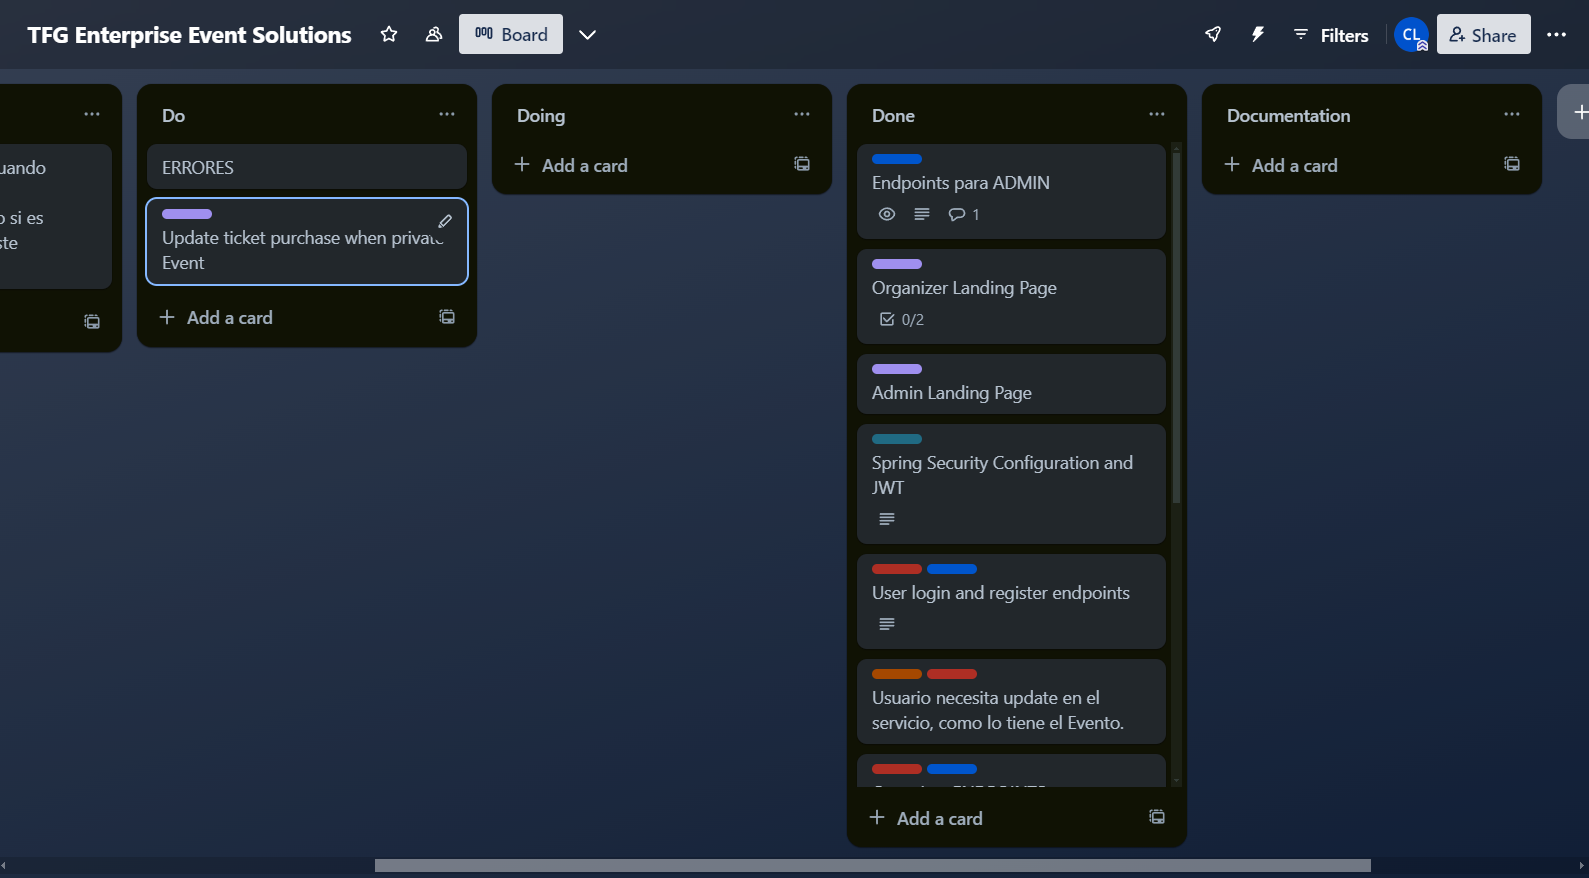
\includegraphics[width=\linewidth]{Trello.png}
    \caption{Trello en proceso.}
    \label{fig:metodologias1}
\end{figure}

En cuanto al desarrollo del código, se ha utilizado un flujo de trabajo basado en Pull Requests (PRs). Cada cambio o nueva 
funcionalidad se desarrollaba en una rama separada y se integraba al código principal solo después de ser revisada y aprobada 
mediante un Pull Request. Este enfoque ha permitido mantener un historial claro de los cambios, realizar revisiones detalladas y 
asegurar que cada nueva adición al código se integrara de manera ordenada y sin conflictos. Este método ha ayudado a mantener la disciplina y la organización en el
 desarrollo del software.

El uso de Pull Requests ha ofrecido múltiples ventajas en el proceso de desarrollo. En primer lugar, ha facilitado la identificación y 
resolución de errores antes de que los cambios se integren en la rama principal. Cada PR actuaba como un punto de control donde podía revisar 
el código, realizar pruebas y verificar la funcionalidad, asegurando que solo los cambios bien testeados y verificados fueran añadidos al proyecto.

Además, este método ha proporcionado una documentación implícita del desarrollo. Cada Pull Request incluía una descripción detallada de los 
cambios realizados, los problemas que solucionaba o las nuevas características añadidas. Esto no solo facilitó la gestión del proyecto, sino 
que también creó un registro histórico útil para futuras referencias y para cualquier otra persona que pueda colaborar en el futuro.

Trabajar con ramas separadas para cada nueva funcionalidad o cambio también ha sido crucial para mantener la estabilidad del proyecto. Al aislar el 
desarrollo de nuevas características en ramas dedicadas, he evitado que los cambios en progreso afecten la estabilidad de la rama principal. Esto ha 
sido especialmente útil para realizar experimentos o implementar grandes cambios sin riesgo de romper la aplicación.

Finalmente, la disciplina de utilizar Pull Requests, incluso trabajando solo, ha fomentado un enfoque metódico y estructurado al desarrollo. Este 
flujo de trabajo me ha obligado a pensar críticamente sobre cada cambio, a documentarlo adecuadamente y a asegurarse de que cada PR cumpliera con los 
estándares de calidad antes de ser fusionado. De hecho, para asegurar que todo cambio que se realizara estuviera controlado por si fuera necesario volver a versiones anteriores
hasta los cambios más pequeños se realizaban mediante PRs. Gracias a esto he consegido revertir cambios en momentos críticos del desarrollo.

\begin{figure}[h]
    \centering
    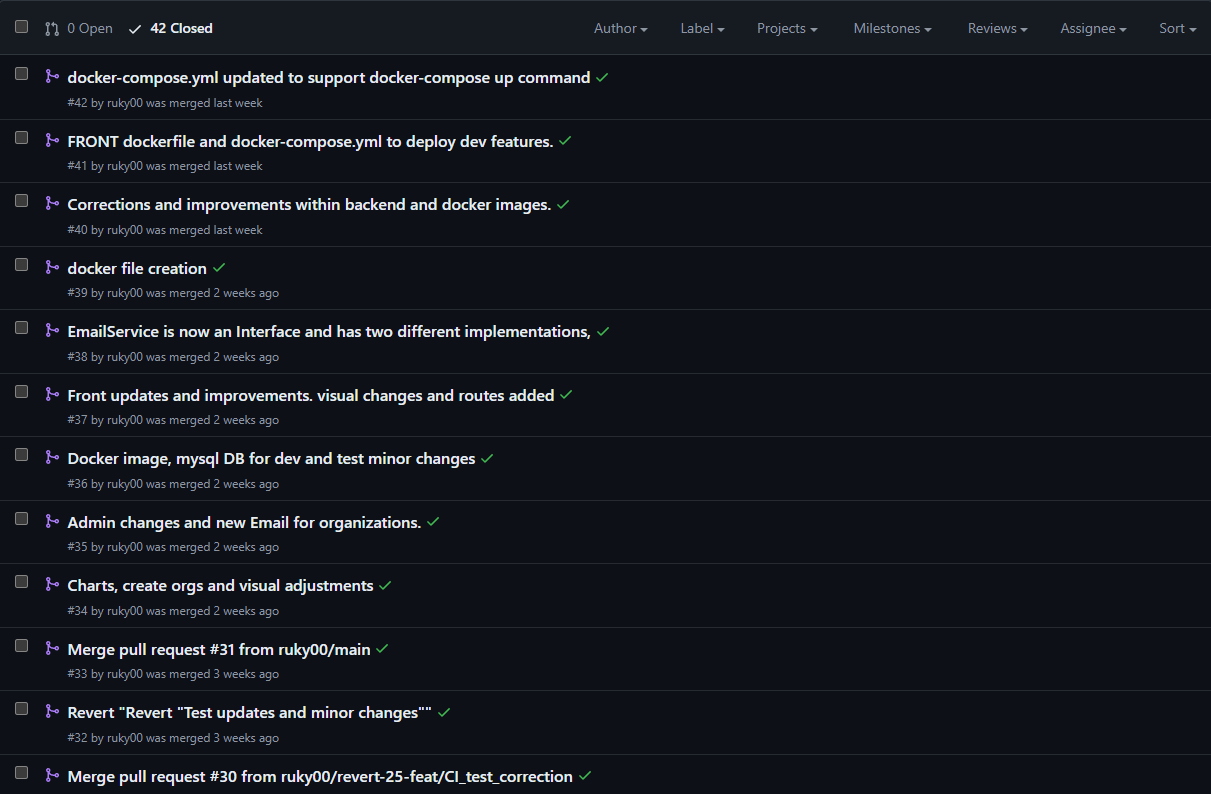
\includegraphics[width=\linewidth]{PRs.png}
    \caption{PRs del Repositorio.}
    \label{fig:metodologias2}
\end{figure}

En resumen, la adopción de la metodología Scrum, con su enfoque en pequeños objetivos semanales y el uso de un tablero Trello para la gestión de tareas, 
junto con el uso de Pull Requests, ha sido clave para el desarrollo exitoso de Enterprise Event Solutions.

El total desarrollo se ha realizado en un repositorio de GitHub donde se ha incluido un Readme.md útil para el tanto el despliegue en producción como en desarrollo. De esta forma
aún sin la totalidad de los requerimientos, ya sea una cuenta de AWS o de Gmail, se podría hacer uso de la aplicación de forma local.




\blankpage

% Capítulo 4
\chapter{Descripción Informática}
\label{chap:contenidos}

En esta sección se entrará a describir con total detalle el contenido técnico de la aplicación. Partiendo desde un analisis de requisitos funcionales
hasta no funcionales, pasando por las tecnologías usadas para la implemetación de estos. 

\section{Tecnologías Empleadas}

\subsection{SpringBoot}
Spring Boot\cite{spring-boot} es un framework Java que simplifica el desarrollo de aplicaciones web al eliminar la 
complejidad de la configuración manual. Ofrece configuración automática, empaquetado de aplicaciones independientes y un inicio rápido integrado, 
lo que permite a los desarrolladores crear aplicaciones de manera más rápida y eficiente, centrándose en la lógica de negocio en lugar de la configuración. 
Genial para el desarrollo de aplicaciones \textit{CRUD}\footnote{\textit{CRUD} es un acrónimo en inglés que se refiere a las operaciones 
básicas de manipulación de datos en aplicaciones informáticas: Create (Crear), Read (Leer), Update (Actualizar) y Delete (Eliminar).}.
\subsection{Maven}
Maven es una herramienta de gestión de proyectos Java que simplifica la estructuración, gestión de dependencias y automatización de la construcción. 
Permite definir dependencias en un archivo de configuración (pom.xml), ejecutar fases de construcción estandarizadas y gestionar repositorios 
centralizados de bibliotecas. Es ampliamente utilizado en el desarrollo Java por su integración con IDEs y su capacidad para proyectos multiproyecto, es decir,
permite la gestión de múltiples proyectos en un solo repositorio, lo que facilita la colaboración entre desarrolladores y la gestión.
\subsection{Vue.js}
Vue.js\cite{vue} es un popular marco de trabajo de código abierto para construir interfaces de usuario interactivas en aplicaciones web de una sola página. 
Se destaca por su enfoque centrado en el componente, su sintaxis declarativa y su eficiente sistema de reactividad. Vue.js facilita la construcción 
de aplicaciones web complejas al fomentar la reutilización de componentes y ofrecer herramientas integradas para la manipulación del DOM y la gestión 
del estado de la aplicación.

\subsection{MySQL}
MySQL es un sistema de gestión de bases de datos relacional de código abierto ampliamente utilizado en el desarrollo de 
aplicaciones web y empresariales. Destaca por su escalabilidad, rendimiento, fiabilidad y facilidad de uso. Ofrece opciones 
sólidas de seguridad y es compatible con una variedad de plataformas y lenguajes de programación. MySQL es una herramienta poderosa 
para gestionar eficientemente grandes volúmenes de datos y garantizar la integridad y disponibilidad de la información.

\subsection{IntelliJ}
IntelliJ IDEA es un entorno de desarrollo integrado (IDE) altamente productivo desarrollado por JetBrains. 
Diseñado para diversas tecnologías, ofrece una interfaz de usuario intuitiva y funciones avanzadas que mejoran la 
productividad del desarrollador. Con soporte para múltiples lenguajes y marcos de trabajo, integración con herramientas de desarrollo y 
características colaborativas, IntelliJ IDEA es una opción popular para el desarrollo de software en Java y otros lenguajes.

\subsection{VSCode}
Visual Studio Code (VSCode) es un IDE popular desarrollado por Microsoft, conocido por su versatilidad, rendimiento y comunidad activa.
 Ofrece características avanzadas y extensiones para diferentes lenguajes de programación. Es altamente personalizable y cuenta con una 
 amplia documentación disponible en su sitio web oficial.

\subsection{AWS S3}
AWS S3 es un servicio de almacenamiento en la nube ofrecido por Amazon Web Services. Destaca por su escalabilidad, durabilidad, seguridad y 
facilidad de uso. Permite almacenar grandes cantidades de datos de forma segura y acceder a ellos de manera eficiente a través de una interfaz 
intuitiva y una API robusta. Con una estructura de precios flexible, AWS S3 es una opción atractiva para empresas que buscan una solución de 
almacenamiento en la nube rentable y confiable.

\subsection{AWS EC2}
AWS EC2 es un servicio de cómputo en la nube proporcionado por Amazon Web Services. Destaca por su escalabilidad, flexibilidad y seguridad. 
Permite a los usuarios alquilar capacidad informática según sus necesidades, con opciones de pago por uso. Es fácil de usar y ofrece una variedad 
de opciones de implementación. En resumen, EC2 es una solución eficiente y confiable para ejecutar aplicaciones y cargas de trabajo en la nube.

\subsection{Docker}
Docker\cite{Docker} es una plataforma de código abierto que permite crear, implementar y ejecutar aplicaciones en contenedores. Destaca por su portabilidad, 
eficiencia y facilidad de uso. Con la tecnología de contenedores, Docker ofrece aislamiento de aplicaciones y escalabilidad, lo que simplifica el 
desarrollo y la administración de aplicaciones en diferentes entornos. En resumen, Docker es una herramienta fundamental para la creación y gestión 
eficiente de aplicaciones modernas.

\newpage
\section{Resumen de las tecnologias}
La Tabla \ref{tabla:tecnologias_usos} recoge un resumen de las tecnologías empleadas para el desarrollo de Enterprise Event Solutions
\begin{table}[h]
\begin{tabular}{ p{3cm} l  }

    \hline
    Tecnologia& Uso \\
    \hline
    SpringBoot   & Framework \\
    Maven &   Framework \\
    Vue.js & Framework  \\
    MySQL    & Tecnologia de BD \\
    IntelliJ&   Entorno de Desarrollo  \\
    VSCode& Entorno de Desarrollo \\
    AWS S3& Tecnologia de de BD en la nube  \\
    AWS EC2& Servidor web en la nube  \\
    Docker& Crecion de imagenes comprimidas para despliegue  \\
    \hline
   \end{tabular}
   \caption{Tecnologías y sus usos correspondientes}
   \label{tabla:tecnologias_usos}
\end{table}
\newpage
\section{Arquitectura}
\textbf{Enterprise Event Solutions} es una aplicación \textbf{Fullstack} creada siguiendo un patrón de diseño MVC. A continuación, se muestra un plano general
que será desglosado:

\section*{Arquitectura General}
\begin{figure}[h]
    \centering
    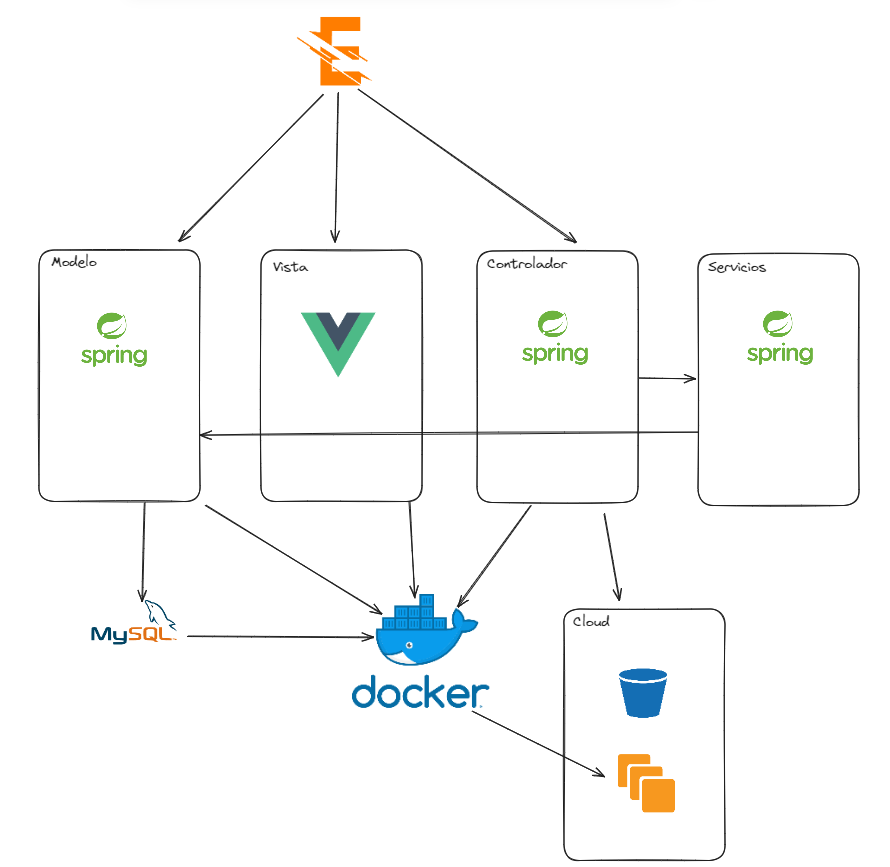
\includegraphics[width=0.8\textwidth]{Arquitectura.png} 
    \caption{Diagrama de Arquitectura de EVS}
    \label{fig:mvc_architecture}
\end{figure}
\newpage

\section*{Backend (Modelo y Controlador)}

\begin{itemize}
    \item \textbf{Tecnología}: \textbf{SpringBoot}
    \item \textbf{Descripción}: Utilizado por su gran versatilidad para manejar la lógica de negocio y control de la aplicación. Gracias a esto, el frontend
    de la aplicación se sirve directamente desde el Servidor de Apache proporcionado por Spring, es decir, tengo empaquetado el tanto el back como el front en la misma ip
    y en el mismo puerto.
\end{itemize}

\section*{Frontend (Vista)}

\begin{itemize}
    \item \textbf{Tecnología}: \textbf{Vue.js}
    \item \textbf{Descripción}: Seleccionado para explorar otras tecnologías y facilitar la creación de una interfaz de usuario interactiva.
\end{itemize}

\section*{Tecnologías Complementarias}

\begin{itemize}
    \item \textbf{AWS EC2}: 
    \begin{itemize}
        \item \textbf{Descripción}: Instancia EC2 para desplegar la aplicación, ofreciendo un entorno robusto y escalable.
    \end{itemize}
    \item \textbf{AWS S3}:
    \begin{itemize}
        \item \textbf{Descripción}: Bucket S3 para almacenar imágenes, reduciendo la carga de trabajo en la base de datos.
    \end{itemize}
    \item \textbf{MySQL}:
    \begin{itemize}
        \item \textbf{Descripción}: Base de datos utilizada para gestionar los datos de la aplicación de manera eficiente.
    \end{itemize}
\end{itemize}

\textbf{Enterprise Event Solutions} combina las fortalezas de \textbf{SpringBoot} y \textbf{Vue.js} en un patrón MVC para ofrecer una solución robusta y 
escalable. Con el soporte de \textbf{AWS} y \textbf{MySQL}, la aplicación está preparada para manejar grandes volúmenes de datos y ofrecer una experiencia 
de usuario fluida.


Cada uno de los componentes definidos en la Imagen \ref{fig:mvc_architecture} será desglosado en las próximas secciones para explicar detalladamente el contenido de 
la aplicación.

\subsection{Modelo}
La persistencia en Enterprise Event Solutions se sustenta en una serie de Entidades almacenadas en una base de datos con la que los servicios interactuan mediante
las interfaces proporcionadas por JPA \ref{sec:jpa}. Es el pilar fundamental en el que se sustenta el modelo de negocio de la aplicación.
\begin{figure}[h]
    \centering
    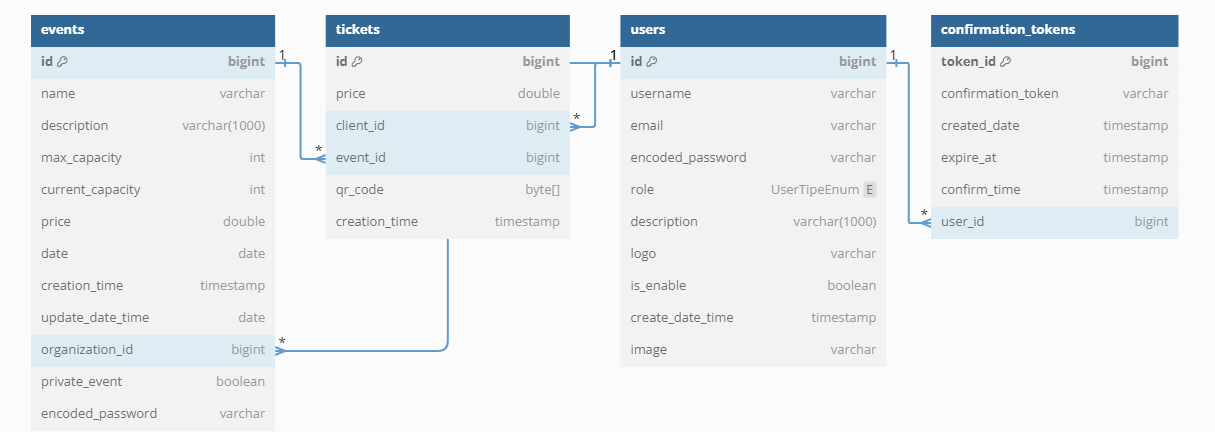
\includegraphics[width=1.2\textwidth]{EVSdiagra.png} 
    \caption{Modelo E-R de la BD}
    \label{fig:diagramaBD}
\end{figure}

\subsubsection{JPA}
\label{sec:jpa}

JPA (Java Persistence API) es una especificación de Java que facilita la gestión de la persistencia de datos en aplicaciones Java.
En Spring, se usa para simplificar las operaciones CRUD y el manejo de relaciones entre entidades, permitiendo trabajar con objetos en lugar de SQL. 
Spring Data JPA integra JPA en el ecosistema Spring, proporcionando repositorios predefinidos para operaciones de base de datos comunes.

A continuación se muestra un fragmento de código de Spring Data JPA en Java:
\myjavastyle
\begin{lstlisting}[language=Java, caption=Ejemplo de Repositorio en Spring Data JPA]
@Repository
public interface UserRepository extends JpaRepository<User,Long> {
    public Optional<User> findByEmail(String email);
    public List<User> findAllByRole(UserTipeEnum type);
    public Optional<User> findByUsername(String username);
}
\end{lstlisting}

Como se puede observar, gracias a la gran potencia de Spring y de JPA, simplemente con crear una interfaz con metodos que creemos que vamos a necesitar en 
nuestros servicios, y sin la necesidad de añadir @Querys, podemos hacer consultas sobre la base de datos.

Pero también podemos hacer nuestras propias Querys sobre la base de datos:
\myjavastyle
\begin{lstlisting}[language=Java, caption=Ejemplo de Query  en Spring Data JPA]
    @Transactional
    @Modifying
    @Query("UPDATE Event e SET e.current_capacity = e.current_capacity + 1 WHERE e.id = :id AND e.current_capacity + 1  <= e.max_capacity")
    public int incrementCurrentCapacity(@Param("id") Long id);
\end{lstlisting}

\subsection{Controlador}
La creación de controladores me ha permitido gestionar un sistema de endpoints que sirve como la interfaz principal 
para la comunicación entre el cliente y el servidor. Estos controladores se encargan de recibir las solicitudes HTTPS de delegar el procesamiento a 
los servicios correspondientes. Los servicios encapsulan la lógica de negocio y se comunican con los repositorios JPA para acceder a los datos de la 
base de datos de manera eficiente. Además, para garantizar la seguridad, se utiliza JWT (JSON Web Tokens), que permite la autenticación y autorización 
de los usuarios. Los tokens JWT se generan tras un inicio de sesión exitoso y se utilizan para proteger los endpoints, asegurando que solo los usuarios 
autenticados puedan acceder a recursos específicos. Este enfoque no solo organiza el código de manera modular y mantenible, sino que también proporciona 
una robusta capa de seguridad para la API.
\begin{figure}[h]
    \centering
    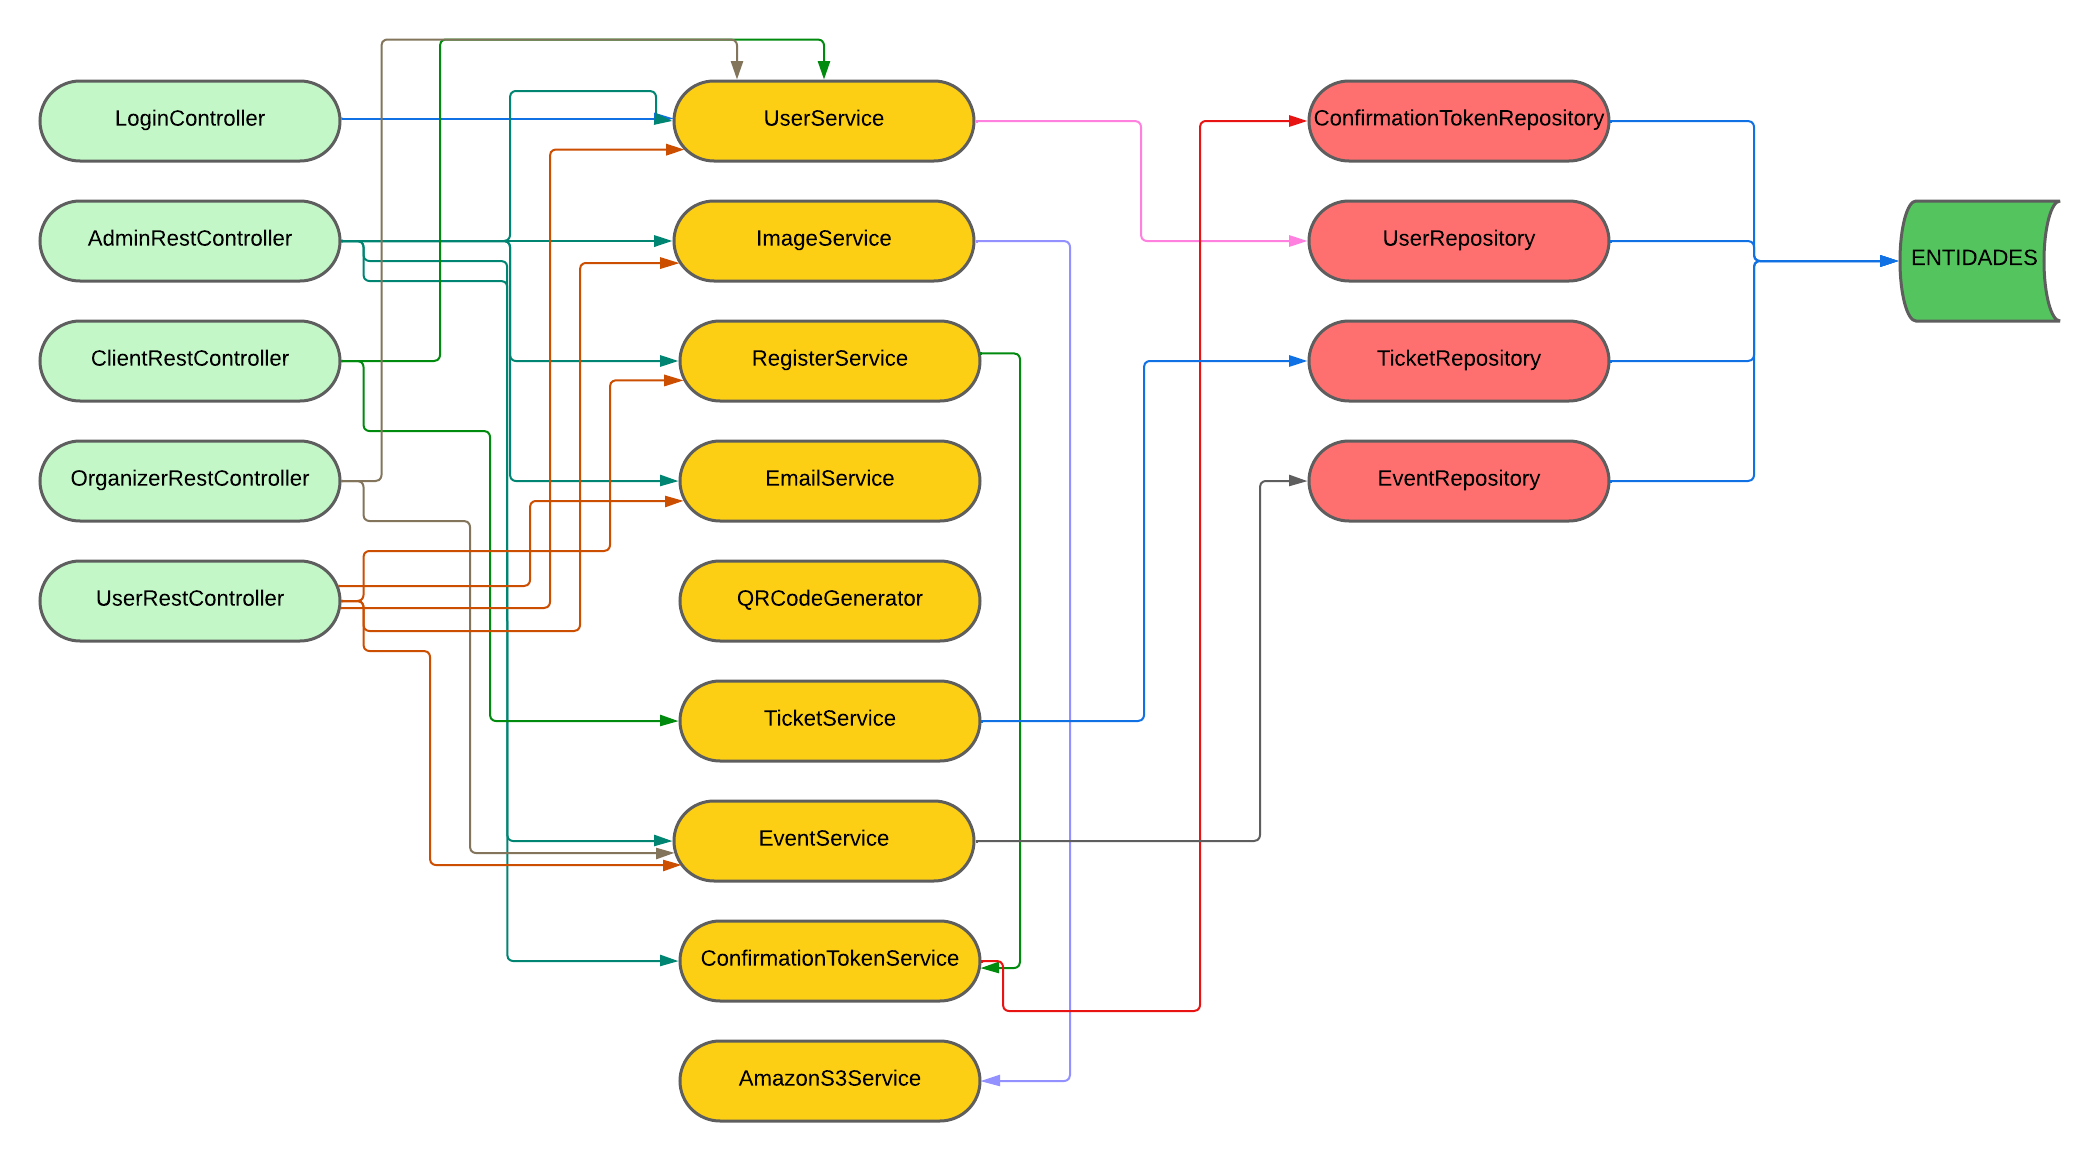
\includegraphics[width=1\textwidth]{DiagramaClases.png} 
    \caption{Diagrama de Clases de EVS}
    \label{fig:class_architecture}
\end{figure}

Además he implementado otras configuraciones para añadir una capa extra de seguridad a la aplicación como configuración CSRFH y Cors para limitar las url 
que pueden hacer uso de los endpoints de mi app. Por supuesto he creado las configuraciones necesarias para manejar las tecnologias externas como S3, dentro de 
EVS.
\begin{figure}[h]
    \centering
    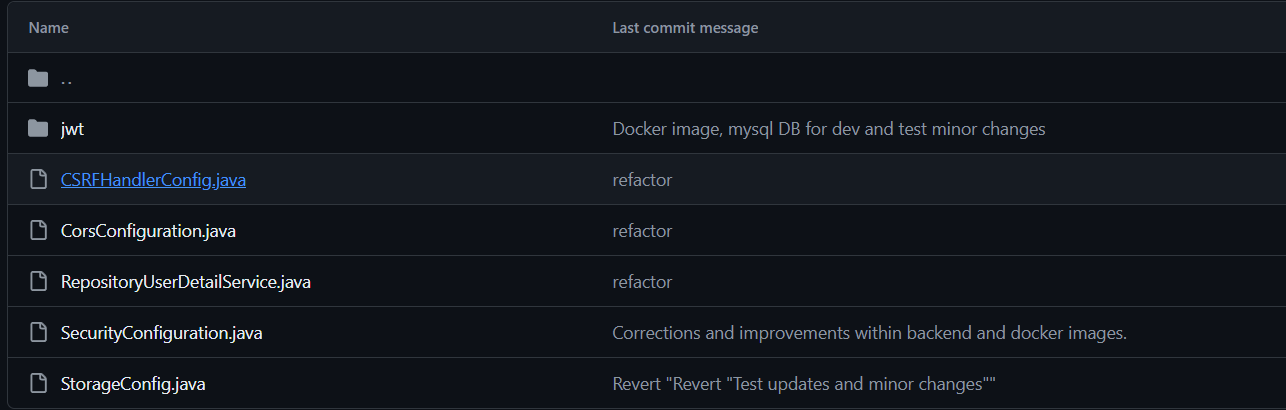
\includegraphics[width=1\textwidth]{security.png} 
    \caption{Seguridad del backend}
    \label{fig:securityClasses}
\end{figure}

\subsection{Vista}
El frontend de Enterprise Event Solutions ha sido implementado en Vue.js. Específicamente en Vue3, que trae consigo algunos cambios con respecto a su versión
anterior Vue2. La utilización de este framework me ha permitido añadir tanto bibliotecas de componentes y gráficos (Bootstrap5 y Chart.js respectivamente)
como relaciones entre los diferentes componentes basado en "props", permitiendo de esta manera diferentes comportamientos del componente dependiendo de
que valores se le pasen en el componente padre.

Un ejemplo del uso de estas props sería:
\myvuestyle
\begin{lstlisting}[language=HTML, caption=Ejemplo del Padre, label=lst:padre]
    <event_cards
    :evento="evento"
    :is-org="false"
    >
    </event_cards>
\end{lstlisting}
\myvuestyle
\begin{lstlisting}[language=HTML, caption=Ejemplo del Hijo, label=lst:hijo]
    <script lang="ts">
    import {EventService} from "../services/event.service";
    import { useRouter } from "vue-router";
    import { Event } from "../models/Event";
    import { computed, ref } from "vue";
    export  default {
        name: "event_cards",
        props:{
          evento: Object as ()=> Event,
          isOrg: Boolean,
        },
    }
\end{lstlisting}

En el código \ref{lst:padre}, se observa que se inserta en el template un componente con la información del evento. Por otro lado, en el código 
\ref{lst:hijo}, se manejan estos valores que hemos pasado desde el componente padre. En este fragmento, si se le pasa \texttt{true} en la variable 
\texttt{is-org}, el componente tendrá un comportamiento diferente a si se le pasa \texttt{false}. Ademas en la variable \texttt{evento} le pasamos la información
del evento para garantizar la reactividad de los componetes de forma individual. De esta forma trabajamos con módulos y no con un elemento.

\newpage
A continuación se muestra un diagrama con las Pantallas de la aplicación y sus acceso en función del tipo de usuario.
\begin{figure}[h]
    \centering
    \rotatebox{90}{
        \includegraphics[width=1\textwidth]{DiagramaFlujo.png}
    }
    \caption{Interfaz con el usuario}
    \label{fig:userInterface}
\end{figure}

\newpage
\subsection{Cloud}
Para mejorar la eficiencia y escalabilidad de la aplicación, he utilizado Amazon S3 para almacenar imágenes y reducir la carga en la base de datos, y 
Amazon EC2 para desplegar la aplicación, garantizando así un rendimiento óptimo y una alta disponibilidad. 

Uno de los objetivos a cumplir era el Despliegue Continuo,es decir, cada vez que realizara un cambio sobre la aplicación se automatizara el proceso 
de despliegue en la maquina EC2. 

Además, este proceso de despliegue automatizado implica una conexión mediante SSH a la instancia de EC2, desde donde se ejecutan los comandos necesarios
para la gestión de contenedores Docker. En resumen, se utiliza GitHub Actions junto con un Runner de la Marketplace para automatizar el despliegue continuo
de nuevas imágenes Docker en una instancia de EC2, asegurando así una actualización constante y sin interrupciones de la aplicación en producción.

\begin{lstlisting}[language=HTML, caption=Action de Automatización CD]
    name: Despliegue en EC2
    
    on:
      workflow_run:
        workflows: ["Construir y Subir Imagen Docker"]
        types:
          - completed
    
    jobs:
      deploy:
        runs-on: ubuntu-latest
        
        steps:
          - name: Execute deployment script on EC2
            uses: easingthemes/ssh-deploy@v5.0.3
            with:
              SSH_PRIVATE_KEY: ${{ secrets.EC2_SSH_KEY }}
              REMOTE_HOST: ${{ secrets.EC2_HOST }}
              REMOTE_USER: ${{ secrets.EC2_USER }}
              
              SCRIPT_AFTER: |
                cd EnterpriseEventSolutions
                sudo ./cd.sh
    \end{lstlisting}
\section{Problemas enfrentados}
Durante la realización del proyecto ha habido que hacer frente a problemas derivados de la falta de conocimiento sobre las herramentas o tecnologías empleadas
por lo que he requerido la ayuda de videos y documentación de las herramientas para poder solventarlo. A continuación hago un resumen de algunos de estos problemas junto con la referencia a sus solución:
\begin{itemize}
    \item  Empaquetado del Frontend erróneo (loading css chunk 323 failed)\cite{cssChunk}: Este error no desplegaba correctamente el front de la aplicación empaquetada.
     Solucioné el error eliminando un import de googleapies.
    \item  Fallo al conectarse a la MySQL(Access denied for user 'root'@'localhost')\cite{mysql}: El error venía de una mala utilización de las .properties de 
     Spring 
\end{itemize}



\section{Especificación de Requisitos}
En esta sección se establecen las necesidades y expectativas a cumplir, así como los elementos clave que guían el diseño y la implementación de la aplicación.

\subsection{Requisitos Funcionales}
La Tabla \ref{tabla:RF} recoge las funcionalidades específicas que el sistema debe ofrecer.

\begin{longtable}{ p{2.5cm} p{4cm} p{9cm}  }
    \caption{Requisitos  Funcionales} \label{tabla:RF} \\
    \hline
    \endfirsthead
    \multicolumn{3}{c}%
    {{\bfseries \tablename\ \thetable{}: Continuación de la tabla anterior}} \\
    \hline
    ID& Resumen& Descripción \\
    \hline
    \endhead
    
    \hline \multicolumn{3}{|r|}{{Continúa en la siguiente página}} \\ \hline
    \endfoot
    
    \hline
    \endlastfoot
    
    \textbf{RF-001}& Login y Registro & El sistema permitirá a los usuarios iniciar sesión con credenciales válidas o registrarse como nuevos 
    usuarios, proporcionando la funcionalidad básica de autenticación y creación de cuentas.\\
    \textbf{RF-002} & Edición completa del perfil por parte de los usuarios & Los usuarios dispondrán de la capacidad total para editar y
    actualizar la información de su perfil dentro del sistema, lo que incluirá datos personales y otros detalles relevantes, ofreciendo una 
    experiencia de usuario personalizada y adaptable.\\
    \textbf{RF-003} & Autorización de correo electrónico & Cuando un usuario se registre, se enviará un correo electrónico de verificación para 
    asegurar la autenticidad de la dirección de correo electrónico proporcionada.\\
    \textbf{RF-101} & Visualización de cantidad de usuarios registrados por mes & El administrador podrá ver la cantidad de usuarios que se han 
    registrado en el sistema durante cada mes.\\
    \textbf{RF-102} & Visualización de cantidad de usuarios por tipo & El administrador podrá ver la cantidad de usuarios registrados clasificados 
    por tipo (administrador, organizador, cliente) en el sistema.\\
    \textbf{RF-103} & Visualización de cantidad de eventos creados por mes & El administrador podrá ver la cantidad de eventos que se han creado en 
    el sistema durante cada mes.\\
    \textbf{RF-104} & Creación de usuarios de tipo Organización & Se dotará al administrador de la capacidad de crear usuarios con el rol específico 
    de 'Organización', lo que permitirá una gestión más detallada y especializada de usuarios dentro del sistema.\\
    \textbf{RF-105} & Filtrado de usuarios por tipo, nombre o email & Se integrará una función que permita al administrador obtener un 
    listado completo de todos los usuarios del sistema, con la posibilidad de aplicar filtros según su tipo de usuario, nombre o dirección 
    de correo electrónico para una búsqueda más eficiente y precisa.\\
    \textbf{RF-106} & Borrado de usuarios por parte del administrador & Se implementará la funcionalidad para que el administrador pueda 
    eliminar usuarios del sistema previa confirmación, permitiendo una gestión eficiente de la base de datos de usuarios y garantizando la integridad 
    y seguridad del sistema.\\
    \textbf{RF-107} & Obtener Usuario en el Sistema & Se implementará la funcionalidad para que el administrador pueda 
    ver información básicas de los usuarios registrados en el sistema\\
    \textbf{RF-108} & Borrado automático & Los usuarios que no hayan confirmado el correo en 15 minutos seran borrados automáticamente del sistema\\
    \textbf{RF-201} & Ver eventos creados por el organizador & El organizador tendrá la capacidad de ver los eventos que ha creado dentro del sistema.\\
    \textbf{RF-202} & Eliminación de eventos por el organizador & Se permitirá al organizador eliminar los eventos que ha creado dentro del sistema.\\
    \textbf{RF-203} & Edición de eventos por el organizador & El organizador podrá editar los eventos que ha creado, lo que incluirá la modificación de 
    detalles como nombre, descripción, fecha, etc.\\
    \textbf{RF-204} & Creación de eventos por el organizador & Se permitirá al organizador crear nuevos eventos proporcionando detalles como nombre, descripción, 
    fecha y, opcionalmente, contraseña para acceder al evento.\\
    \textbf{RF-205} & Visualización de cantidad de inscritos en eventos por el organizador & El organizador podrá ver la cantidad de usuarios inscritos en los 
    eventos que ha creado dentro del sistema.\\
    \textbf{RF-301} & Visualización de organizaciones por parte del cliente & Los clientes tendrán la capacidad de ver las organizaciones disponibles en el sistema.\\
    \textbf{RF-302} & Visualización de perfil de organizaciones por parte del cliente & Los clientes podrán ver el perfil de las organizaciones dentro del sistema.\\
    \textbf{RF-303} & Visualización de eventos de organizaciones por parte del cliente & Los clientes podrán ver los eventos que ofrecen las organizaciones dentro del sistema.\\
    \textbf{RF-304} & Inscripción a eventos por parte del cliente & Los clientes podrán inscribirse a los eventos ofrecidos por las organizaciones dentro del sistema.\\
    \textbf{RF-305} & Eventos privados con contraseña & Se permitirá la creación de eventos privados que requieran una contraseña para acceder a ellos.\\
    \textbf{RF-306} & Generación de entradas para eventos & Una vez adquirida la entrada, se generará un código QR para acceder al evento.\\
    \textbf{RF-307} & Manejo de Concurrencia & En caso de que dos usuarios intenten adquirir una entrada simultáneamente, se debe implementar 
    un sistema de colas para evitar incongruencias en la base de datos. \\
    \textbf{RF-308} & Descarga de PDF de la Entrada & Los Clientes tienen que tener la opción de poder descargar la entrada en formato PDF para poder
    compartirla si quisieran\\
    \end{longtable}
    \newpage
    \subsection{Requisitos No Funcionales}
    La Tabla \ref{tabla:RNF} recoge las funcionalidades para mejorar la experiencia del usuario, se abordan tanto las limitaciones 
    técnicas como los factores a considerar.

    \begin{longtable}{ p{2.5cm} p{4cm} p{9cm} }
        \caption{Requisitos No Funcionales} \label{tabla:RNF} \\
        \hline
        ID & Resumen & Descripción \\
        \hline
        \endfirsthead
        \multicolumn{3}{c}{{\bfseries \tablename\ \thetable{}: Continuación de la tabla anterior}} \\
        \hline
        ID & Resumen & Descripción \\
        \hline
        \endhead
        \hline \multicolumn{3}{|r|}{{Continúa en la siguiente página}} \\ \hline
        \endfoot
        \hline
        \endlastfoot
        \textbf{RNF-001} & Desempeño del sistema & El sistema debe ser capaz de manejar hasta 1000 usuarios simultáneos sin experimentar una degradación 
        significativa del rendimiento. \\
        \textbf{RNF-002} & Seguridad de los datos & Todos los datos sensibles almacenados en el sistema deben estar cifrados utilizando un algoritmo de cifrado 
        estándar. \\
        \textbf{RNF-003} & Usabilidad & La interfaz de usuario debe ser intuitiva y fácil de usar, con tiempos de carga de página inferiores a 1 segundo para 
        mejorar la experiencia del usuario. \\
        \textbf{RNF-004} &  Conexión a Internet & El sistema debe tener acceso a Internet para permitir la comunicación con servicios externos y el intercambio
         de datos. \\
        \textbf{RNF-005} & Rendimiento & El sistema debe responder a las solicitudes del usuario dentro de un tiempo aceptable, con tiempos de carga de página y
         operaciones de procesamiento mínimos. \\
        \textbf{RNF-006} & Accesibilidad & Tiene que ser posible usar la aplicación de forma óptima en dispositivos móviles\\ 
    \end{longtable}

\section{Pruebas}
En esta sección, se presentan las pruebas realizadas para asegurar que todos los requisitos se cumplen correctamente y que no hay errores durante la ejecución del 
sistema. Se incluyen descripciones detalladas de los diferentes test llevados a cabo, así como los resultados obtenidos, con el objetivo de validar el 
funcionamiento y la estabilidad del software.

Se han realizado tanto pruebas REST como pruebas Unitarias. No se han realizado pruebas de Interfaz.

\subsection{Pruebas REST}
Las pruebas REST son pruebas de software que validan la funcionalidad de las API RESTful, asegurando que los endpoints, métodos HTTP, respuestas y códigos de 
estado funcionen correctamente.

Para la realización de las pruebas REST se ha incluido tambien las pruebas de Integración. Cada vez que se realice un conjunto de test, se realiza la conexión con 
un contenedor Docker con una imagen MySQL de la misma versión que la utilizada en la aplicación para garantizar el correcto funcionamiento sobre esta Base de Datos.


\begin{itemize}
    \item \textbf{Descripción de la prueba:} Verificar que un usuario no registrado puede crear un usuario Cliente.
    \item \textbf{Trazabilidad:} RF-001.
    \item \textbf{Precondiciones:} La aplicación debe estar en ejecución y disponible para recibir solicitudes API.
    \item \textbf{Acciones:}
    \begin{enumerate} 
        \item Crear un nuevo usuario con el rol de 'Client' enviando una solicitud POST a la API con los datos del usuario.
        \item Comprobar que la respuesta HTTP es 201 (Created).
    \end{enumerate}
    \item \textbf{Resultados esperados:}
    \begin{itemize}
        \item El servidor debe responder con un código de estado HTTP 201 (Created) indicando que el usuario ha sido creado correctamente.
        \item La información del nuevo usuario debe ser almacenada en la base de datos.
    \end{itemize}
    \item \textbf{Incidencias:}
    \begin{itemize}
        \item OK. La prueba fue exitosa, el usuario fue creado y la respuesta del servidor fue 201 (Created).
    \end{itemize}
\end{itemize}

\begin{itemize}
    \item \textbf{Descripción de la prueba:} Verificar que un usuario no registrado puede crear un usuario Organizador/Cliente y luego iniciar sesión correctamente.
    \item \textbf{Trazabilidad:} RF-001.
    \item \textbf{Precondiciones:} La aplicación debe estar en ejecución y disponible para recibir solicitudes API.
    \item \textbf{Acciones:}
    \begin{enumerate}
        \item Crear un nuevo usuario con el rol de 'Organizer' o 'Client' enviando una solicitud POST a la API con los datos del usuario.
        \item Comprobar que la respuesta HTTP es 201 (Created) y que el usuario se ha creado correctamente.
        \item Iniciar sesión con el usuario creado enviando una solicitud POST a la API con las credenciales del usuario.
        \item Comprobar que la respuesta HTTP es 200 (OK) y que la respuesta indica un inicio de sesión exitoso.
    \end{enumerate}
    \item \textbf{Resultados esperados:}
    \begin{itemize}
        \item El servidor debe responder con un código de estado HTTP 201 (Created) al crear el usuario, indicando que el usuario ha sido creado correctamente.
        \item La información del nuevo usuario debe ser almacenada en la base de datos.
        \item El servidor debe responder con un código de estado HTTP 200 (OK) al iniciar sesión, indicando un inicio de sesión exitoso.
        \item La respuesta de inicio de sesión debe contener un campo 'status' con el valor "SUCCESS".
    \end{itemize}
    \item \textbf{Incidencias:}
    \begin{itemize}
        \item OK. La prueba fue exitosa, el usuario fue creado y pudo iniciar sesión correctamente.
    \end{itemize}
\end{itemize}

\begin{itemize}
    \item \textbf{Descripción de la prueba:} Registrarse para un evento.
    \item \textbf{Trazabilidad:} RF-304.
    \item \textbf{Precondiciones:} El sistema debe estar en ejecución y disponible para recibir solicitudes API.
    \item \textbf{Acciones:}
    \begin{enumerate}
        \item Simular un usuario autenticado con el rol de 'CLIENT'.
        \item Enviar una solicitud POST a la API para registrar al usuario en un evento específico.
        \item Verificar que la respuesta HTTP es 201 (Created), lo que indica que la inscripción fue exitosa.
    \end{enumerate}
    \item \textbf{Resultados esperados:}
    \begin{itemize}
        \item El servidor debe responder con un código de estado HTTP 201 (Created), indicando que la inscripción al evento fue exitosa.
    \end{itemize}
    \item \textbf{Incidencias:}
    \begin{itemize}
        \item OK. La prueba fue exitosa, el usuario se inscribió correctamente.
    \end{itemize}
\end{itemize}

\begin{itemize}
    \item \textbf{Descripción de la prueba:} Verificar que un usuario puede ver sus entradas.
    \item \textbf{Trazabilidad:} RF-306, RF-304.
    \item \textbf{Precondiciones:} El sistema debe estar en ejecución y disponible para recibir solicitudes API.
    \item \textbf{Acciones:}
    \begin{enumerate}
        \item Simular un usuario autenticado con el rol de 'CLIENT'.
        \item Enviar una solicitud GET a la API para obtener las entradas del usuario.
        \item Verificar que la respuesta HTTP es 200 (OK) y que la respuesta es un arreglo JSON, lo que indica que las entradas del usuario se recuperaron correctamente.
    \end{enumerate}
    \item \textbf{Resultados esperados:}
    \begin{itemize}
        \item El servidor debe responder con un código de estado HTTP 200 (OK), indicando que la solicitud fue exitosa.
        \item La respuesta debe ser un arreglo JSON, que contiene las entradas del usuario.
    \end{itemize}
    \item \textbf{Incidencias:}
    \begin{itemize}
        \item OK. La prueba fue exitosa, el usuario obtuvo la información de sus entradas.
    \end{itemize}
\end{itemize}

\begin{itemize}
    \item \textbf{Descripción de la prueba:} Verificar que un usuario puede ver las organizaciones a las que está asociado.
    \item \textbf{Trazabilidad:} RF-301.
    \item \textbf{Precondiciones:} El sistema debe estar en ejecución y disponible para recibir solicitudes API.
    \item \textbf{Acciones:}
    \begin{enumerate}
        \item Simular un usuario autenticado con el rol de 'CLIENT'.
        \item Enviar una solicitud GET a la API para obtener las organizaciones asociadas al usuario.
        \item Verificar que la respuesta HTTP es 200 (OK) y que la respuesta es un arreglo JSON, lo que indica que las organizaciones se recuperaron correctamente.
    \end{enumerate}
    \item \textbf{Resultados esperados:}
    \begin{itemize}
        \item El servidor debe responder con un código de estado HTTP 200 (OK), indicando que la solicitud fue exitosa.
        \item La respuesta debe ser un arreglo JSON, que contiene las organizaciones asociadas al usuario.
    \end{itemize}
    \item \textbf{Incidencias:}
    \begin{itemize}
        \item OK. La prueba fue exitosa, el usuario obtuvo la información de las organizaciones.
    \end{itemize}
\end{itemize}

\begin{itemize}
    \item \textbf{Descripción de la prueba:} Verificar que un organizador puede publicar un nuevo evento en el sistema.
    \item \textbf{Trazabilidad:} RF-204.
    \item \textbf{Precondiciones:} El sistema debe estar en ejecución y disponible para recibir solicitudes API.
    \item \textbf{Acciones:}
    \begin{enumerate}
        \item Simular un usuario autenticado con el rol de 'ORGANIZATION'.
        \item Crear un nuevo evento con los detalles especificados y convertirlo a formato JSON.
        \item Enviar una solicitud POST a la API para publicar el evento.
        \item Verificar que la respuesta HTTP es 201 (Created), indicando que el evento se creó correctamente.
    \end{enumerate}
    \item \textbf{Resultados esperados:}
    \begin{itemize}
        \item El servidor debe responder con un código de estado HTTP 201 (Created), indicando que el evento se ha creado correctamente.
    \end{itemize}
    \item \textbf{Incidencias:}
    \begin{itemize}
        \item OK. La prueba fue exitosa, el usuario pudo crear Eventos.
    \end{itemize}
\end{itemize}

\begin{itemize}
    \item \textbf{Descripción de la prueba:} Verificar que un organizador puede eliminar un evento existente del sistema.
    \item \textbf{Trazabilidad:} RF-202.
    \item \textbf{Precondiciones:} El sistema debe estar en ejecución y disponible para recibir solicitudes API. Además, debe existir al menos un evento en la base de datos.
    \item \textbf{Acciones:}
    \begin{enumerate}
        \item Simular un usuario autenticado con el rol de 'ORGANIZER'.
        \item Obtener la lista de eventos disponibles.
        \item Verificar que la respuesta HTTP es 200 (OK) y que contiene al menos un evento.
        \item Identificar el ID del primer evento en la lista para eliminarlo.
        \item Enviar una solicitud DELETE a la API para eliminar el evento utilizando su ID.
        \item Verificar que la respuesta HTTP es 200 (OK), indicando que el evento se eliminó correctamente.
    \end{enumerate}
    \item \textbf{Resultados esperados:}
    \begin{itemize}
        \item El servidor debe responder con un código de estado HTTP 200 (OK), indicando que el evento se ha eliminado correctamente.
    \end{itemize}
    \item \textbf{Incidencias:}
    \begin{itemize}
        \item OK. La prueba fue exitosa, el usuario pudo eliminar un Evento.
    \end{itemize}
\end{itemize}


\subsection{Pruebas Unitarias}
Las pruebas unitarias se realizan para garantizar que partes específicas del código funcionen como se espera, sin depender de otras partes del sistema. 
Esto ayuda a detectar errores temprano, asegurar la calidad del código, facilitar la refactorización y proporcionar documentación sobre el comportamiento esperado del 
código.

A continuación, se muestran las PU correspondientes a los requsitos que no se han probado con pruebas REST para ampliar la covertura del código.

\begin{itemize}
    \item \textbf{Descripción de la prueba:} Verificar que todos los eventos de un organizador pueden ser obtenidos.
    \item \textbf{Trazabilidad:} RF-201.
    \item \textbf{Precondiciones:} El usuario debe estar autenticado como 'Carlos' con el rol de 'CLIENT'.
    \item \textbf{Acciones:}
    \begin{enumerate}
        \item Configurar el comportamiento del mock de UserService para que devuelva el organizador cuando se llame a findByUsername con el argumento 'URJC'.
        \item Configurar el comportamiento del mock de EventService para que devuelva una lista falsa de eventos cuando se llame a findByUser con el organizador.
        \item Realizar una solicitud GET a la API para obtener los eventos, especificando el parámetro 'org' como 'URJC'.
        \item Verificar que la respuesta HTTP es 200 (OK) y que el cuerpo de la respuesta contiene una lista de eventos con un tamaño de 2.
        \item Verificar que se llamó al método findByUser en EventService con el organizador como argumento.
    \end{enumerate}
    \item \textbf{Resultados esperados:}
    \begin{itemize}
        \item Se espera que la solicitud obtenga una respuesta con estado HTTP 200 (OK).
        \item Se espera una lista de tamaño 2.
    \end{itemize}
    \item \textbf{Incidencias:}
    \begin{itemize}
        \item OK. La prueba fue existosa.
    \end{itemize}
\end{itemize}

\begin{itemize}
    \item \textbf{Descripción de la prueba:} Verificar que un evento puede ser obtenido por su ID.
    \item \textbf{Trazabilidad:} RF-303.
    \item \textbf{Precondiciones:} El usuario debe estar autenticado como 'Carlos' con el rol de 'CLIENT'.
    \item \textbf{Acciones:}
    \begin{enumerate}
        \item Configurar el comportamiento del mock de EventService para que devuelva el evento1 cuando se llame a findById con el argumento 1L.
        \item Realizar una solicitud GET a la API para obtener el evento con ID 1.
        \item Verificar que la respuesta HTTP es 200 (OK) y que el cuerpo de la respuesta contiene el evento con ID 1.
        \item Verificar que se llamó al método findById en EventService con el argumento 1L.
    \end{enumerate}
    \item \textbf{Resultados esperados:}
    \begin{itemize}
        \item Se espera que la solicitud obtenga una respuesta con estado HTTP 200 (OK).
        \item Se espera que contenga el evento con ID 1.
    \end{itemize}
    \item \textbf{Incidencias:}
    \begin{itemize}
        \item OK. La prueba fue existosa.
    \end{itemize}
\end{itemize}

\begin{itemize}
    \item \textbf{Descripción de la prueba:} Verificar que todos los usuarios pueden ser obtenidos por un administrador.
    \item \textbf{Trazabilidad:} RF-107.
    \item \textbf{Precondiciones:} El usuario debe estar autenticado como 'Admin' con el rol de 'ADMIN'.
    \item \textbf{Acciones:}
    \begin{enumerate}
        \item Configurar el comportamiento del mock de UserService para que devuelva una lista de usuarios falsos cuando se llame a findAll.
        \item Realizar una solicitud GET a la API para obtener todos los usuarios.
        \item Verificar que la respuesta HTTP es 200 (OK) y que el cuerpo de la respuesta contiene una lista de usuarios con al menos 2 elementos.
        \item Verificar que se llamó al método findAll en UserService.
    \end{enumerate}
    \item \textbf{Resultados esperados:}
    \begin{itemize}
        \item Se espera que la solicitud obtenga una respuesta con estado HTTP 200 (OK) 
        \item Se espera que contenga una lista de usuarios con al menos 2 elementos.
    \end{itemize}
    \item \textbf{Incidencias:}
    \begin{itemize}
        \item OK. La prueba fue existosa.
    \end{itemize}
\end{itemize}
\newpage
\section{Flujo de la Aplicación}

En esta sección se presenta el diagrama de flujo de la aplicación dividida en partes para su mejor comprensión.
\begin{figure}[h]
    \centering
    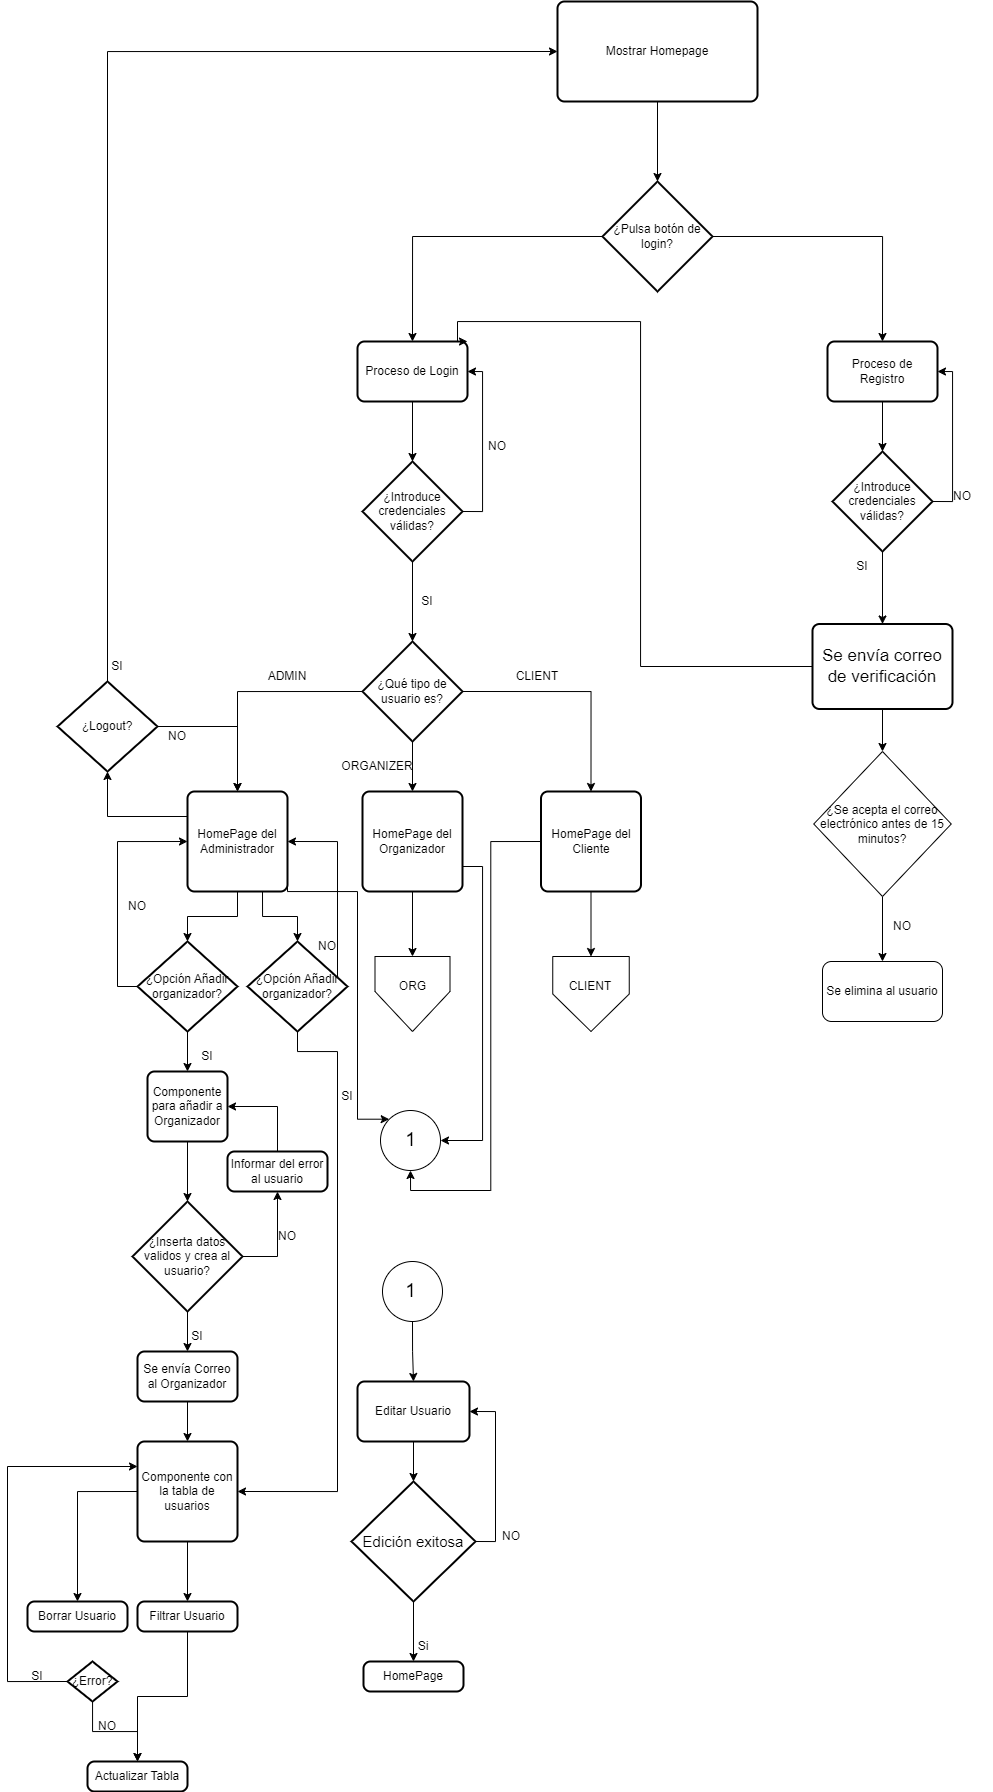
\includegraphics[width=0.9\textwidth]{FlujoEVS1.png} 
    \caption{Diagrama de Flujo Parte 1}
    \label{fig:flujoEvs}
\end{figure}
\newpage
\begin{figure}[h]
    \centering
    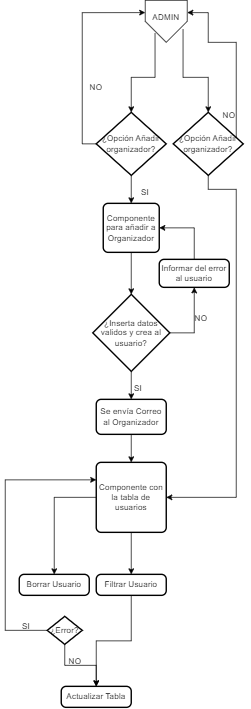
\includegraphics[width=0.4\textwidth]{AdminFlujo.png} 
    \caption{Diagrama de Flujo Parte 2}
    \label{fig:flujoEvs1}
\end{figure}
\newpage
\begin{figure}[h]
    \centering
    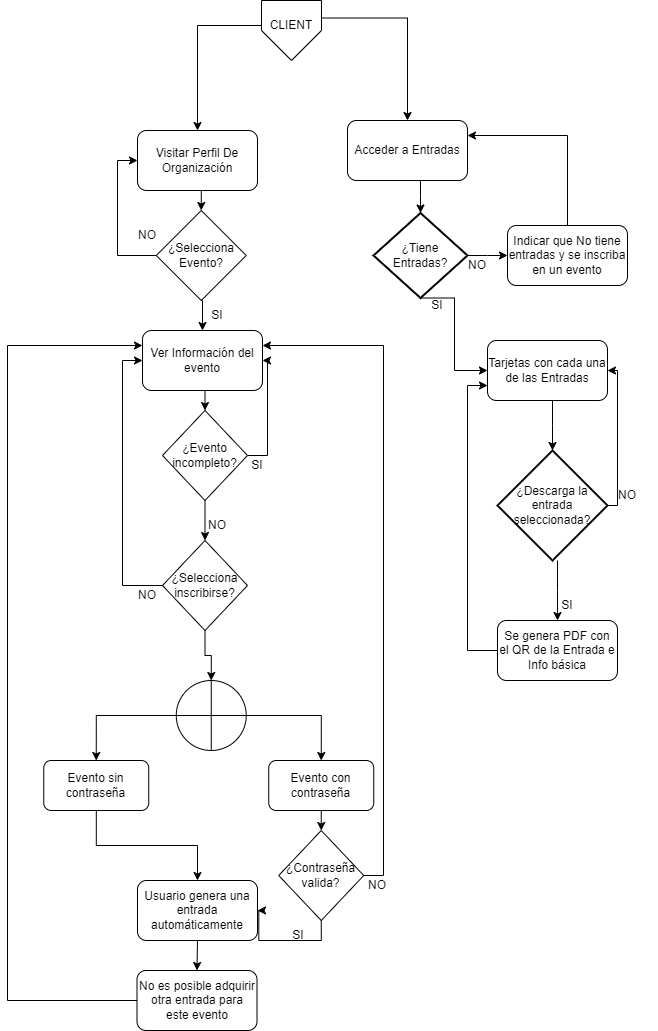
\includegraphics[width=0.7\textwidth]{Cliente.png} 
    \caption{Diagrama de Flujo Parte 3}
    \label{fig:flujoEvs2}
\end{figure}
\newpage
\begin{figure}[h]
    \centering
    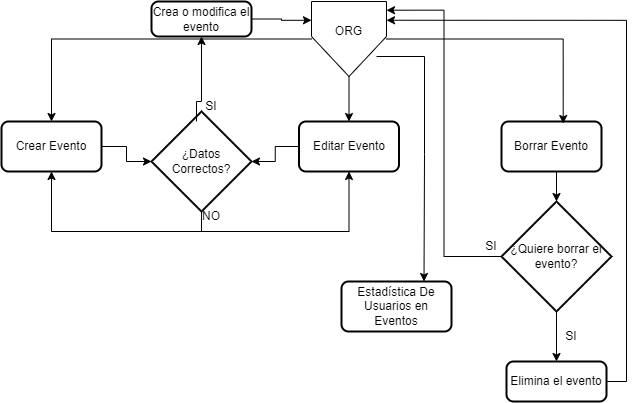
\includegraphics[width=0.8\textwidth]{Org.png} 
    \caption{Diagrama de Flujo Parte 4}
    \label{fig:flujoEvs3}
\end{figure}



\section{Estudio de Caso}
Dado que Enterprise Event Solutions es una aplicación diseñada para usuarios comunes, se ha llevado a cabo un estudio para recopilar opiniones y percepciones
 sobre la aplicación. En este estudio se incluyen preguntas tanto antes como después del uso de la aplicación por parte de los usuarios. Para la recolección de datos, 
 se utilizó Google Forms, y los resultados obtenidos se presentan en la sección de Apéndice.

\subsection{Perfil de los Participantes}
Debido a que la aplicaciones tiene diferentes tipos de usuarios he optado por seleccionar una serie de estos participantes para que interactuaran como organizadores,
como clientes o como administradores. En total se ha evaluado a 10 Participantes.
Cabe destacar que para la primera interacción con la aplicación se le ha requerido al Participante realizar una serie de pasos en la aplicación para 
valorar posteriormente la \textbf{usabilidad} y \textbf{accesibilidad} de esta.

\subsection{Valoración general}
A la pregunta "¿Darías uso a esta aplicación?" se obtuvo una puntuación de 4.25 sobre 5, lo que indica un éxito generalizado de Enterprise Event Solutions.
Esta valoración sugiere una aceptación positiva y una disposición favorable hacia la aplicación, con solo un participante atípico que se desvió de la opinión
general.

\subsection{Desempeño}

De forma general, la evaluación de este aspecto es positiva, aunque es importante destacar algunos comentarios sobre la responsividad de la página. Este problema
fue corregido tan pronto como se identificó el error.

\subsection{Diseño, Usabilidad y Accesibilidad}
En las primeras versiones de la aplicación, se observó que la interfaz gráfica carecía de ciertas facilidades para la navegación, como elementos
identificativos, códigos QR, flechas de navegación, spinners de carga y pantallas de error adecuadas. Además, el diseño dificultaba su uso, lo que llevó a una reestructuración completa de la página.

Es importante destacar que estos comentarios se recopilaron a lo largo del ciclo de vida del proyecto, y no únicamente en su etapa final.
Por lo tanto, considero que el contacto continuo con el usuario final es fundamental para lograr un producto refinado.


En rasgos generales los Participantes consideran Enterprise Event Solutions una aplicación sencilla y no tienen ningún problema para entender ninguna de las
funcionalidades.


\blankpage

% Nuevo capítulo

\chapter{Conclusiones y trabajos futuros}

\tutor{Mejor darle la vuelta siguiendo el orden del título, ¿no crees?}
\section{Futuros Proyectos}
Como creador de Enterprise Event Solutions, y el significado que tiene para mí, tengo intención de continuar mejorando Enterprise Event Solutions hasta
su límite. Algunas funcionalidades extra que podría incluir serían:
\begin{itemize}
    \item Software de lectura de QR integrada: Validar las entradas desde la propia aplicación para poder acceder al evento.
    \item Pasarela de pago: Los eventos que sean de pago puedan ser abonados desde la propia aplicación. 
    \item Ampliar el sistema de Correo: Añadir correos de alerta cuando se aproxima la fecha de un evento.
\end{itemize}

Las posibilidades con una aplicación de este tipo son infinitas. Estas son algunas de las posibles mejoras a corto-medio plazo. 

\section{Conclusiones}
Pese a que ya existen numerosas aplicaciones para gestionar eventos, he querido darle otro enfoque centrado en el la gente de a pie y en las pequeñas empresas,
EVS permite concentrar la gestión de clientes y eventos en un mismo sitio ahorrando infinidad de recursos tanto materiales como personales. 

La gran aceptación que ha tenido entre los participantes del Estudio de Caso es para mí una recompensa al esfuerzo y las horas dedicadas a este TFG, y por supuesto
me animan a continuar con el desarrollo.

Por otro lado me gustaría recalcar que, gracias a realizar este proyecto, he adquirido conocimientos útiles para el desarrollo laboral y personal y por 
supuesto no se quedará ahí ya que he descubierto que cada vez me gusta más el mundo del Desarrollo de Aplicaciones Web aunque si me tengo que decantar, me quedo con
el Backend.


\blankpage


%%%%%%%%%%%%%%%%%%%%%%%%%%%%%%% Bibliografía %%%%%%%%%%%%%%%%%%%%%%%%%%%%%%%

\phantomsection
\addcontentsline{toc}{chapter}{Bibliografía}

\footnotesize{
%\bibliographystyle{hispa}
\bibliographystyle{IEEEtran}
\bibliography{bibliografia}
}



% No expandir elementos para llenar toda la página
\raggedbottom
\afterpage{\blankpage}

\newpage




%%%%%%%%%%%%%%%%%%%%%%%%%%%%%%% Apéndices %%%%%%%%%%%%%%%%%%%%%%%%%%%%%%%

\appendix

\phantomsection
\addcontentsline{toc}{chapter}{Apéndices}

\mbox{}
\vfill
\begin{center}
\begin{Huge}
\textbf{Apéndices}
\end{Huge}
\end{center}
\vfill
\mbox{}
\thispagestyle{empty}

\newpage
\mbox{}
\thispagestyle{empty}
\newpage


% Primer apéndice
\chapter{Estudio de Caso}
\label{sec:apendice1}

\section{Formulario Estudio de Caso}

A continuación se muestran los datos recogidos del Estudio de Caso: 
\tutor{Parece muy completo, pero las preguntas deben definirse en la memoria (y ya redirigir aquí para las respuestas completas}
\textbf{\href{https://forms.gle/vdjaMq6vTJrPTLeh7}{Enlace a Formulario EVS}}

\begin{figure}[h]
    \centering
    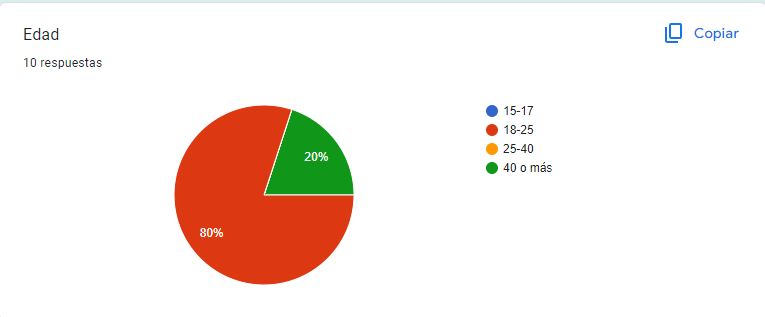
\includegraphics[width=0.9\textwidth]{Form1.png} 
    \caption{Formulario Pregunta 1}
    \label{fig:form1}
\end{figure}
\begin{figure}[h]
    \centering
    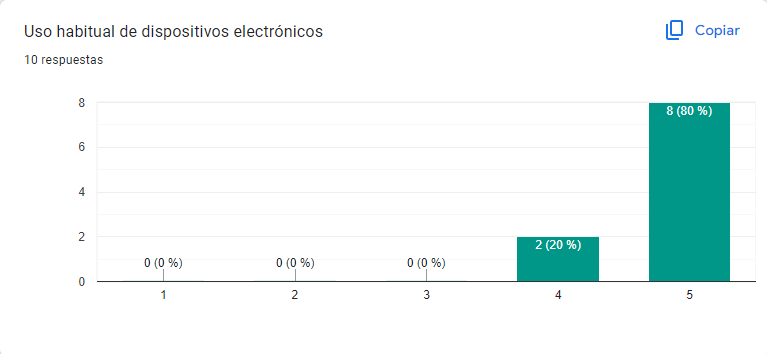
\includegraphics[width=0.9\textwidth]{Form2.png} 
    \caption{Formulario Pregunta 2}
    \label{fig:form2}
\end{figure} 
\begin{figure}[h]
    \centering
    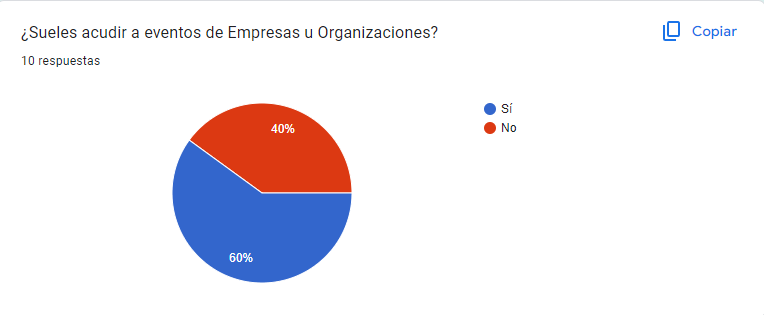
\includegraphics[width=0.9\textwidth]{Form3.png} 
    \caption{Formulario Pregunta 3}
    \label{fig:form3}
\end{figure}
\begin{figure}[h]
    \centering
    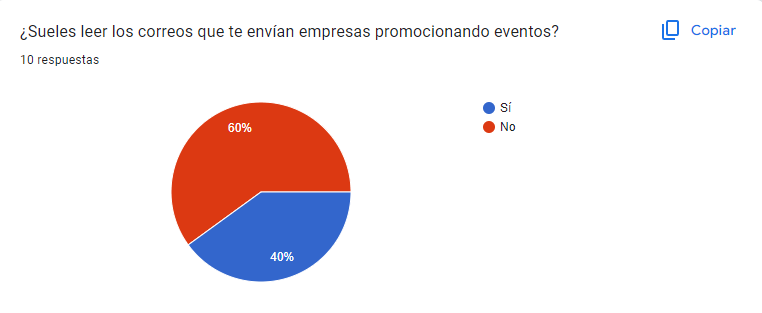
\includegraphics[width=0.9\textwidth]{Form4.png} 
    \caption{Formulario Pregunta 4}
    \label{fig:form4}
\end{figure}
\begin{figure}[h]
    \centering
    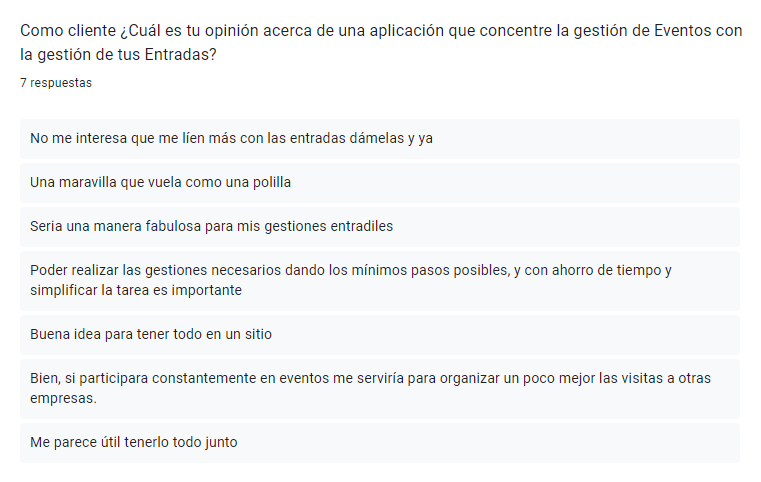
\includegraphics[width=0.9\textwidth]{Form5.png} 
    \caption{Formulario Pregunta 5}
    \label{fig:form5}
\end{figure}
\begin{figure}[h]
    \centering
    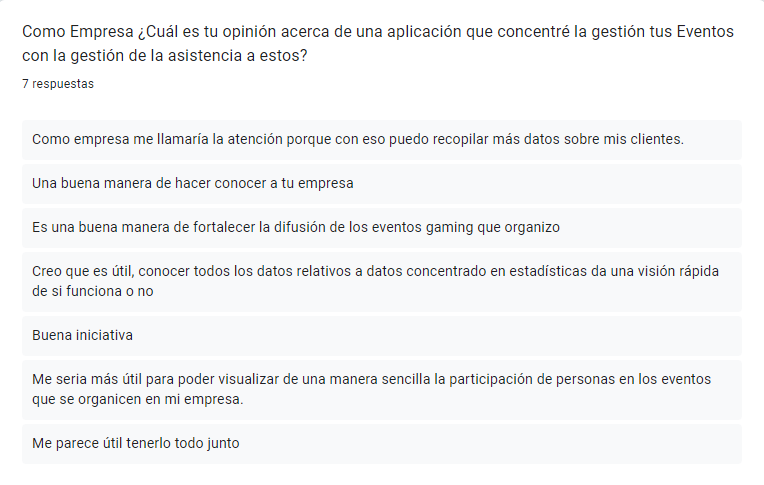
\includegraphics[width=0.9\textwidth]{Form6.png} 
    \caption{Formulario Pregunta 6}
    \label{fig:form6}
\end{figure}
\begin{figure}[h]
    \centering
    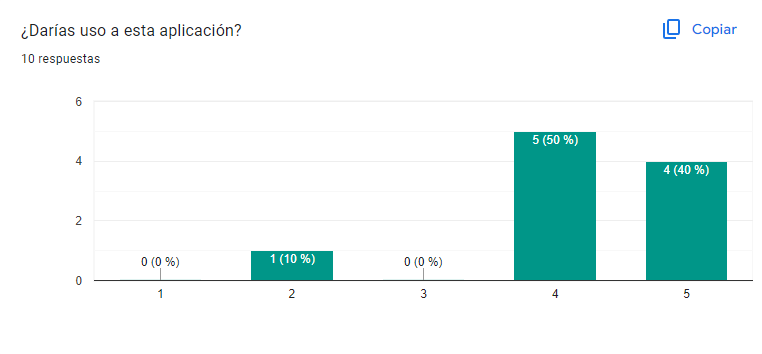
\includegraphics[width=0.9\textwidth]{Form7.png} 
    \caption{Formulario Pregunta 7}
    \label{fig:form7}
\end{figure}
\begin{figure}[h]
    \centering
    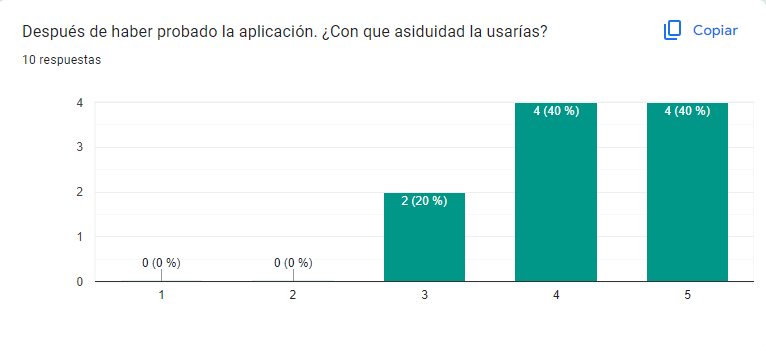
\includegraphics[width=0.9\textwidth]{Form8.png} 
    \caption{Formulario Pregunta 8}
    \label{fig:form8}
\end{figure}
\begin{figure}[h]
    \centering
    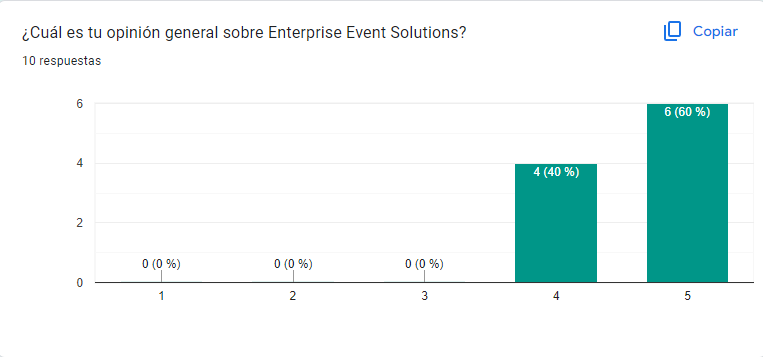
\includegraphics[width=0.9\textwidth]{Form9.png} 
    \caption{Formulario Pregunta 9}
    \label{fig:form9}
\end{figure}


% Segundo apéndice
\chapter{Lanzamiento en Local}
\label{sec:apendice2}

\section{Requisitos}
Se recomienda de disponer un sistema operativo Linux o en su defecto un subsistema Linux dentro de nuestro propio ordenador.
    \begin{itemize}
        \item  \textbf{Docker}:Para instalar Docker sigue las instrucciones de su página principal.\footnote{\href{https://docs.docker.com/get-docker/}{https://docs.docker.com/get-docker/}} 
        \item  \textbf{npm y Node.js}Para el frontend es necesario estas dos programas. Se pueden instalar desde su sitio oficial.\footnote{\href{https://docs.npmjs.com/downloading-and-installing-node-js-and-npm}{https://docs.npmjs.com/downloading-and-installing-node-js-and-npm}} 
    \end{itemize}
\section{Lanzamiento en producción}
Para lanzar la aplicación hay que seguir los siguientes pasos:
\subsection{Clonar repositorio de Github}
\begin{lstlisting}[language=Bash, caption=Script clonar repositorio, label=lst:clonarRepo]
git clone https://github.com/ruky00/EnterpriseEventSolutions.git
cd EnterpriseEventSolutions
\end{lstlisting}

\subsection{Construir imagen Docker}
Ejecuta el siguiente comando:
\begin{lstlisting}[language=Bash, caption=Crear imagen Docker, label=lst:constImagen]
docker build -t evsglobal -f multistage-dockerfile.Dockerfile .
\end{lstlisting}

En caso de querer automatizar este proceso, hay un script .sh creado en la carpeta 'backend' que crea y sube al repositorio de DockerHub una nueva versión de la aplicación.

\subsection{Lanzar aplicación en producción}
w
\subsubsection{Variables de entorno}
Para poder hacer uso de la aplicación en un entorno local en producción hay que definir las variables de entorno de las tecnologías de apoyo para la aplicación, S3 y servicio de correo:
\begin{itemize}
    \item AWS\_ACCESS\_KEY\_ID: \${AWS\_ACCESS\_KEY\_ID}
    \item AWS\_SECRET\_ACCESS\_KEY: \${AWS\_SECRET\_ACCESS\_KEY}
    \item AWS\_REGION: \${AWS\_REGION}
    \item EMAIL\_TFG: \${EMAIL\_TFG}
    \item EMAIL\_SERVICE: \${EMAIL\_SERVICE}
\end{itemize}

\subsubsection{docker-compose}
Finalmente se ejecuta comando 'docker-compose up' que lanzará las imagenes tanto de la base de datos MySQL como la imagen con la última versión de la aplicación.
\begin{lstlisting}[language=Bash, caption=Lanzar contenedores Docker, label=lst:docker-compose]
version: '3.8'
services:

  mysql:
    image: mysql:8.0.28
    container_name: evs1
    environment:
      - MYSQL_DATABASE=evs
      - MYSQL_ROOT_PASSWORD=password
    ports:
      - "3306:3306"
    restart: on-failure

  app_prod:
    image: ruky00/evsglobal
    ports:
      - "8443:8443"
    environment:
      - SPRING_PROFILES_ACTIVE=prod
      - SPRING_DATASOURCE_URL=jdbc:mysql://evs1:3306/evs
      - SPRING_DATASOURCE_USERNAME=root
      - SPRING_DATASOURCE_PASSWORD=password
      - AWS_ACCESS_KEY_ID=${AWS_ACCESS_KEY_ID}
      - AWS_SECRET_ACCESS_KEY=${AWS_SECRET_ACCESS_KEY}
      - AWS_REGION=${AWS_REGION}
      - EMAIL_TFG=${EMAIL_TFG}
      - EMAIL_SERVICE=${EMAIL_SERVICE}
    depends_on:
      - mysql
    restart: on-failure


\end{lstlisting}

\subsubsection{Verificar que la aplicación funciona}
Abre el navegador y accede a la dirección \href{https://localhost:8443}{https://localhost:8443}. En caso de que salte alguna advertencia de seguridad, desestímala y continua a la app.

\section{Lanzar aplicación en desarrollo}
En el caso de querer hacer uso de la aplicación sin necesidad de tener una cuenta de AWS ni un correo electrónico, se puede lanzar la aplicación con una versión en desarrollo que
carece de las dependencias de S3 y de correo electrónico. 

Además de esta forma se pueden realizar cambios en cada una de las secciones de la app sin tener que parar la totalidad de la aplicación. 

\subsubsection{Ejecutar backend}
Ejecuta los comandos \ref{lst:devBuild} para construir el ejecutable de la aplicación.
\begin{lstlisting}[language=Bash, caption=Construir ejecutable, label=lst:devBuild]
cd backend
mvn package
\end{lstlisting}

Una vez finalizada la ejecución de los test se creará un archivo .jar. Ejecuta el comando \ref{lst:devBuildJAr} para lanzar el backend.
\begin{lstlisting}[language=Bash, caption=Lanzar ejecutable, label=lst:devBuildJAr]
java -jar "-Dspring.profiles.active=dev" .\target\EnterPriseEventSolutions-0.0.1-SNAPSHOT.jar
\end{lstlisting}

\subsubsection{Ejecutar frontend}
Por otro lado tenemos que lanzar el fortend. En primer lugar instalamos las dependencias.
\begin{lstlisting}[language=Bash, caption=Instalar dependencias del frontend, label=lst:frontBuild]
cd frotend/EnterPriseEventSolutions
npm i
\end{lstlisting}

Y ejecutamos el comando \ref{lst:frontServe} para lanzar el front en desarollo y poder realizar cambios que se verán al momento.
\begin{lstlisting}[language=Bash, caption=Lanzar frontend, label=lst:frontServe]
npm run serve
\end{lstlisting}

\subsubsection{Verificar correcto funcionamiento}
Abre el navegador y accede a la dirección \href{http://localhost:8080}{http://localhost:8080} que es donde esta alojado el frontend para verificar que el front funciona correctamente.
y hacemos un post de un usuario nuevo para verificar la conexión con el backend.


\section{Usuarios de Prueba}
Para acceder a la aplicación y probar las diferentes características de esta se tiene que hacer con una serie de usuarios con los permisos correspondientes.
\begin{itemize}
    \item Usuario Administrador: usuario: admin@admin.com contraseña:pass
    \item Usuario Organización: usuario: inaki@example.com contraseña:pass
    \item Usuario Cliente: usuario: michel@example.com contraseña:pass
\end{itemize}

% Tercer apéndice
\chapter{Enlace a Enterprise Event Solutions}
\label{sec:apendice3}

\section{Enlace a la aplicación}
Se puede hacer uso de la aplicación accediendo al siguiente enlace: \textbf{\href{https://18.133.60.104:8443/}{https://18.133.60.104:8443/}}




% Fin del documento
\end{document}
